% Select document class: uncomment one of the following
\documentclass[aspectratio=169]{beamer}  % For presentation mode
%\documentclass[11pt]{article}            % For article mode
%\usepackage{beamerarticle}               % Uncomment with article class

% =============================================================================
% COMMON PREAMBLE
% =============================================================================
% =============================================================================
% Common Preamble for Network+ Lecture Series
% This file provides consistent formatting, colors, packages, and styles
% across all lecture modules for both beamer presentations and article mode
% =============================================================================

% =============================================================================
% THEME AND COLORS
% =============================================================================
\usetheme{Madrid}
\usecolortheme{whale}

% Custom colors - standardized across all lectures
\definecolor{rctcblue}{RGB}{0, 74, 136}
\definecolor{rctcgold}{RGB}{255, 199, 44}
\definecolor{networkgreen}{RGB}{0, 128, 64}
\definecolor{alertred}{RGB}{180, 0, 0}
\definecolor{aborange}{RGB}{230, 126, 34}
\definecolor{copperbrown}{RGB}{184, 115, 51}
\definecolor{faborange}{RGB}{255, 165, 0}
\definecolor{fiberyellow}{RGB}{255, 215, 0}
\definecolor{shirepurple}{RGB}{102, 51, 153}
\definecolor{ipblue}{RGB}{52, 152, 219}
\definecolor{ippurple}{RGB}{155, 89, 182}
\definecolor{vlangreen}{RGB}{39, 174, 96}
\definecolor{tcpblue}{RGB}{30, 100, 180}
\definecolor{udpgreen}{RGB}{50, 160, 80}
\definecolor{dhcppurple}{RGB}{120, 60, 160}
\definecolor{dnsyellow}{RGB}{200, 170, 50}
\definecolor{batblack}{RGB}{30, 30, 40}
\definecolor{gothamgray}{RGB}{80, 85, 95}
\definecolor{paddysgreen}{RGB}{19, 77, 33}
\definecolor{beerlight}{RGB}{255, 199, 44}
\definecolor{sunnyorange}{RGB}{255, 140, 0}
\definecolor{ogregreen}{RGB}{34, 139, 34}
\definecolor{swampbrown}{RGB}{101, 67, 33}

% Set theme colors
\setbeamercolor{palette primary}{bg=rctcblue,fg=white}
\setbeamercolor{palette secondary}{bg=rctcblue!80,fg=white}
\setbeamercolor{palette tertiary}{bg=rctcblue!60,fg=white}
\setbeamercolor{structure}{fg=rctcblue}
\setbeamercolor{title}{fg=white,bg=rctcblue}
\setbeamercolor{frametitle}{fg=white,bg=rctcblue}
\setbeamercolor{block title}{bg=rctcblue,fg=white}
\setbeamercolor{block body}{bg=rctcblue!10,fg=black}
\setbeamercolor{block title alerted}{bg=alertred,fg=white}
\setbeamercolor{block body alerted}{bg=alertred!10,fg=black}
\setbeamercolor{block title example}{bg=networkgreen,fg=white}
\setbeamercolor{block body example}{bg=networkgreen!10,fg=black}

% =============================================================================
% PACKAGES
% =============================================================================
\usepackage[utf8]{inputenc}
\usepackage[T1]{fontenc}
\usepackage{lmodern}  % Better font rendering
\usepackage{graphicx}
\usepackage{tikz}
\usepackage{booktabs}
\usepackage{array}
\usepackage{multirow}
\usepackage{hyperref}
\usepackage{adjustbox}
\usepackage{amssymb}
\usepackage{amsmath}
\usepackage{calc}
\usepackage{fontawesome5}
% xcolor with [table] option: avoid colortbl.4ht hook conflict in tex4ht
\ifdefined\HCode
  \usepackage{xcolor}
  \usepackage{colortbl}  % provides \rowcolor etc.
\else
  \usepackage[table]{xcolor}  % includes colortbl for pdflatex
\fi

% =============================================================================
% TIKZ LIBRARIES AND SETUP
% =============================================================================
\usetikzlibrary{
    shapes.geometric,
    shapes.symbols,
    shapes.misc,
    arrows.meta,
    positioning,
    calc,
    fit,
    backgrounds,
    decorations.pathreplacing,
    decorations.pathmorphing,
    matrix,
    chains
}
% shadows library causes pgfuseshading errors with tex4ht;
% only load it when NOT building HTML
\ifdefined\HCode\else
    \usetikzlibrary{shadows}
\fi

% Graphics path for icons and chapter images
\graphicspath{
    {../images/icons/}
    {./images/icons/}
    {images/icons/}
    {../images/ch1/}
    {./images/ch1/}
    {images/ch1/}
    {../images/ch2/}
    {./images/ch2/}
    {images/ch2/}
    {../images/ch3/}
    {./images/ch3/}
    {images/ch3/}
    {../images/ch4/}
    {./images/ch4/}
    {images/ch4/}
    {../images/ch5/}
    {./images/ch5/}
    {images/ch5/}
    {../images/ch6/}
    {./images/ch6/}
    {images/ch6/}
    {../images/ch7/}
    {./images/ch7/}
    {images/ch7/}
    {../images/ch8/}
    {./images/ch8/}
    {images/ch8/}
    {../images/ch9/}
    {./images/ch9/}
    {images/ch9/}
    {../images/}
    {./images/}
    {images/}
}

% =============================================================================
% NETWORK DIAGRAM STYLES
% =============================================================================
\tikzset{
    % Node styles for network devices
    device/.style={
        inner sep=2pt,
        label distance=2pt
    },
    pc/.style={device},
    laptop/.style={device},
    server/.style={device},
    router/.style={device},
    switch/.style={device},
    firewall/.style={device},
    cloud/.style={device},
    phone/.style={device},
    tablet/.style={device},
    wifi/.style={device},
    % Connection styles
    ethernet/.style={
        draw=rctcblue,
        line width=1.5pt,
        -{Stealth[length=3mm]}
    },
    ethernet noarrow/.style={
        draw=rctcblue,
        line width=1.5pt
    },
    wireless/.style={
        draw=aborange,
        line width=1.5pt,
        dashed,
        -{Stealth[length=3mm]}
    },
    wireless noarrow/.style={
        draw=aborange,
        line width=1.5pt,
        dashed
    },
    wan/.style={
        draw=alertred,
        line width=2pt,
        -{Stealth[length=3mm]}
    },
    wan noarrow/.style={
        draw=alertred,
        line width=2pt
    },
    copper/.style={
        draw=copperbrown,
        line width=2pt,
        -{Stealth[length=3mm]}
    },
    copper noarrow/.style={
        draw=copperbrown,
        line width=2pt
    },
    fiber/.style={
        draw=fiberyellow,
        line width=2pt,
        -{Stealth[length=3mm]}
    },
    fiber noarrow/.style={
        draw=fiberyellow,
        line width=2pt
    },
    trunk/.style={
        draw=shirepurple,
        line width=2pt,
        -{Stealth[length=3mm]}
    },
    trunk noarrow/.style={
        draw=shirepurple,
        line width=2pt
    },
    % Packet/segment styles
    pktseg/.style={
        draw=rctcblue,
        fill=rctcblue!10,
        minimum height=0.5cm,
        font=\tiny,
        rounded corners=2pt
    },
    pktseg tcp/.style={
        draw=tcpblue,
        fill=tcpblue!15,
        minimum height=0.5cm,
        font=\tiny,
        rounded corners=2pt
    },
    pktseg udp/.style={
        draw=udpgreen,
        fill=udpgreen!15,
        minimum height=0.5cm,
        font=\tiny,
        rounded corners=2pt
    },
    pktseg highlight/.style={
        draw=aborange,
        fill=aborange!20,
        minimum height=0.5cm,
        font=\tiny,
        rounded corners=2pt
    },
    % Box styles
    ipbox/.style={
        draw=rctcblue,
        fill=rctcblue!10,
        rounded corners,
        minimum height=0.4cm,
        font=\small
    },
    portbox/.style={
        draw=tcpblue,
        fill=tcpblue!10,
        rounded corners,
        minimum height=0.4cm,
        font=\small
    },
    dnsbox/.style={
        draw=dnsyellow,
        fill=dnsyellow!15,
        rounded corners,
        minimum height=0.4cm,
        font=\small
    },
    routetable/.style={
        draw=rctcblue,
        fill=rctcblue!10,
        rounded corners,
        minimum height=0.4cm,
        font=\small
    },
    macbox/.style={
        draw=networkgreen,
        fill=networkgreen!10,
        rounded corners,
        minimum height=0.4cm,
        font=\small
    },
    % Frame segment styles (Ethernet frame diagrams)
    frameseg/.style={
        draw=rctcblue,
        fill=rctcblue!10,
        minimum height=0.5cm,
        font=\tiny,
        rounded corners=2pt
    },
    frameseg highlight/.style={
        draw=aborange,
        fill=aborange!20,
        minimum height=0.5cm,
        font=\tiny,
        rounded corners=2pt
    },
    % Process/flow styles
    process/.style={
        draw=rctcblue,
        fill=rctcblue!15,
        rounded corners,
        minimum width=2cm,
        minimum height=0.6cm,
        font=\small,
        align=center
    },
    decision/.style={
        draw=aborange,
        fill=aborange!15,
        diamond,
        aspect=2,
        minimum width=1.5cm,
        font=\small,
        align=center
    },
    % OSI Layer styles
    osilayer/.style={
        draw=rctcblue,
        fill=rctcblue!10,
        minimum width=3cm,
        minimum height=0.45cm,
        font=\small
    },
    osilayer highlight/.style={
        draw=aborange,
        fill=aborange!20,
        line width=1.5pt,
        minimum width=3cm,
        minimum height=0.45cm,
        font=\small\bfseries
    }
}

% =============================================================================
% ICON COMMANDS - Standardized using PNG files and FontAwesome
% =============================================================================
% Network device icons (PNG)
\newcommand{\iconpc}[1][0.6cm]{\resizebox{#1}{!}{
\includegraphics{icon_pc}}}
\newcommand{\iconlaptop}[1][0.6cm]{\resizebox{#1}{!}{
\includegraphics{icon_laptop}}}
\newcommand{\iconserver}[1][0.6cm]{\resizebox{#1}{!}{
\includegraphics{icon_server}}}
\newcommand{\iconrouter}[1][0.6cm]{\resizebox{#1}{!}{
\includegraphics{icon_router}}}
\newcommand{\iconswitch}[1][0.6cm]{\resizebox{#1}{!}{
\includegraphics{icon_switch}}}
\newcommand{\iconfirewall}[1][0.6cm]{\resizebox{#1}{!}{
\includegraphics{icon_firewall}}}
\newcommand{\iconcloud}[1][0.6cm]{\resizebox{#1}{!}{
\includegraphics{icon_cloud}}}
\newcommand{\iconphone}[1][0.6cm]{\resizebox{#1}{!}{
\includegraphics{icon_phone}}}
\newcommand{\icontablet}[1][0.6cm]{\resizebox{#1}{!}{
\includegraphics{icon_tablet}}}
\newcommand{\iconwifi}[1][0.6cm]{\resizebox{#1}{!}{
\includegraphics{icon_wifi}}}
\newcommand{\icondatabase}[1][0.6cm]{\resizebox{#1}{!}{
\includegraphics{icon_db}}}
\newcommand{\iconlock}[1][0.6cm]{\resizebox{#1}{!}{
\includegraphics{icon_lock}}}

% For HTML/tex4ht builds: replace PNG icons with FontAwesome5 glyphs.
% dvisvgm embeds font glyphs as vectors but silently ignores em:graph (PNG)
% specials, so PNG icons would be blank in the output SVGs. FA5 glyphs work.
\ifdefined\HCode
  \renewcommand{\iconpc}[1][0.6cm]{\resizebox{#1}{!}{\faIcon{desktop}}}
  \renewcommand{\iconlaptop}[1][0.6cm]{\resizebox{#1}{!}{\faIcon{laptop}}}
  \renewcommand{\iconserver}[1][0.6cm]{\resizebox{#1}{!}{\faIcon{server}}}
  \renewcommand{\iconrouter}[1][0.6cm]{\resizebox{#1}{!}{\faIcon{route}}}
  \renewcommand{\iconswitch}[1][0.6cm]{\resizebox{#1}{!}{\faIcon{network-wired}}}
  \renewcommand{\iconfirewall}[1][0.6cm]{\resizebox{#1}{!}{\faIcon{shield-alt}}}
  \renewcommand{\iconcloud}[1][0.6cm]{\resizebox{#1}{!}{\faIcon{cloud}}}
  \renewcommand{\iconphone}[1][0.6cm]{\resizebox{#1}{!}{\faIcon{mobile-alt}}}
  \renewcommand{\icontablet}[1][0.6cm]{\resizebox{#1}{!}{\faIcon{tablet-alt}}}
  \renewcommand{\iconwifi}[1][0.6cm]{\resizebox{#1}{!}{\faIcon{wifi}}}
  \renewcommand{\icondatabase}[1][0.6cm]{\resizebox{#1}{!}{\faIcon{database}}}
  \renewcommand{\iconlock}[1][0.6cm]{\resizebox{#1}{!}{\faIcon{lock}}}
\fi

% FontAwesome icons
\newcommand{\iconuser}[1][0.6cm]{\resizebox{#1}{!}{\faIcon{user}}}
\newcommand{\iconglobe}[1][0.6cm]{\resizebox{#1}{!}{\faIcon{globe}}}
\newcommand{\iconclock}[1][0.6cm]{\resizebox{#1}{!}{\faIcon{clock}}}
\newcommand{\iconmail}[1][0.6cm]{\resizebox{#1}{!}{\faIcon{envelope}}}
\newcommand{\icondoc}[1][0.6cm]{\resizebox{#1}{!}{\faIcon{file-alt}}}
\newcommand{\iconsearch}[1][0.6cm]{\resizebox{#1}{!}{\faIcon{search}}}
\newcommand{\icontools}[1][0.6cm]{\resizebox{#1}{!}{\faIcon{tools}}}
\newcommand{\iconchart}[1][0.6cm]{\resizebox{#1}{!}{\faIcon{chart-line}}}
\newcommand{\iconalert}[1][0.6cm]{\resizebox{#1}{!}{\faIcon{bell}}}
\newcommand{\iconlog}[1][0.6cm]{\resizebox{#1}{!}{\faIcon{clipboard-list}}}
\newcommand{\iconeye}[1][0.6cm]{\resizebox{#1}{!}{\faIcon{eye}}}
\newcommand{\iconhacker}[1][0.6cm]{\resizebox{#1}{!}{\faIcon{user-secret}}}
\newcommand{\iconkey}[1][0.6cm]{\resizebox{#1}{!}{\faIcon{key}}}
\newcommand{\iconfile}[1][0.6cm]{\resizebox{#1}{!}{\faIcon{file-alt}}}
\newcommand{\icondog}[1][0.6cm]{\resizebox{#1}{!}{\faIcon{dog}}}
\newcommand{\iconcat}[1][0.6cm]{\resizebox{#1}{!}{\faIcon{cat}}}
\newcommand{\iconvoip}[1][0.6cm]{\resizebox{#1}{!}{\faIcon{phone-volume}}}
\newcommand{\iconmoney}[1][0.6cm]{\resizebox{#1}{!}{\faIcon{money-bill-wave}}}
\newcommand{\icontrash}[1][0.6cm]{\resizebox{#1}{!}{\faIcon{trash}}}
\newcommand{\iconbuilding}[1][0.6cm]{\resizebox{#1}{!}{\faIcon{building}}}

% =============================================================================
% CUSTOM COMMANDS AND ENVIRONMENTS
% =============================================================================

% Key term formatting
\newcommand{\keyterm}[1]{\textbf{#1}}

% Slide section marker
\newcommand{\sectionslide}[1]{
    \begin{frame}
        \vfill
        \centering
        \begin{beamercolorbox}[sep=8pt,center,shadow=true,rounded=true]{title}
            \usebeamerfont{title}\Huge #1
        \end{beamercolorbox}
        \vfill
    \end{frame}
}

% Case study frame environment
\newenvironment{casestudy}[1]{%
    \begin{alertblock}{$\blacktriangleright$ Case Study: #1}
}{%
    \end{alertblock}
}

% Solution frame environment  
\newenvironment{casesolution}[1]{%
    \begin{exampleblock}{$\checkmark$ Solution: #1}
}{%
    \end{exampleblock}
}

% =============================================================================
% FOOTER WITH SLIDE NUMBERS
% =============================================================================
\setbeamertemplate{footline}{
    \leavevmode%
    \hbox{%
        \begin{beamercolorbox}[wd=.333333\paperwidth,ht=2.25ex,dp=1ex,center]{author in head/foot}%
            \usebeamerfont{author in head/foot}\insertshortauthor
        \end{beamercolorbox}%
        \begin{beamercolorbox}[wd=.333333\paperwidth,ht=2.25ex,dp=1ex,center]{title in head/foot}%
            \usebeamerfont{title in head/foot}\insertshorttitle
        \end{beamercolorbox}%
        \begin{beamercolorbox}[wd=.333333\paperwidth,ht=2.25ex,dp=1ex,right]{date in head/foot}%
            \usebeamerfont{date in head/foot}\insertshortdate{}\hspace*{2em}
            \insertframenumber{} / \inserttotalframenumber\hspace*{2ex}
        \end{beamercolorbox}}%
    \vskip0pt%
}

% =============================================================================
% ARTICLE MODE SUPPORT
% =============================================================================
% The following commands help with beamerarticle mode for HTML conversion

% In article mode, add proper section/subsection support and override environments
\mode<article>{
    % Make sure figure captions work properly
    \setbeamertemplate{caption}[numbered]
    \setbeamertemplate{caption label separator}{: }
    
    % Add some spacing for readability
    \setlength{\parskip}{0.5em}
    \setlength{\parindent}{0pt}
    
    % Article mode versions of case study environments
    \renewenvironment{casestudy}[1]{%
        \vspace{0.3cm}\noindent\textbf{Case Study: #1}\newline\begin{itshape}
    }{%
        \end{itshape}\vspace{0.3cm}
    }
    
    \renewenvironment{casesolution}[1]{%
        \vspace{0.3cm}\noindent\textbf{Solution: #1}\newline\begin{itshape}
    }{%
        \end{itshape}\vspace{0.3cm}
    }
}

% Command to mark content that only appears in article mode
\newcommand{\articleonly}[1]{\mode<article>{#1}}

% Command to mark content that only appears in presentation mode
\newcommand{\presentationonly}[1]{\mode<presentation>{#1}}


% =============================================================================
% DOCUMENT INFO
% =============================================================================
\title[Module 6.0]{Module 6.0: Implementing Network Services}
\subtitle{Intro to Networks}
\author{Brendan Shea, PhD}
\date{Introduction to Networking}

\mode<article>{
\let\originaltikzpicture\tikzpicture
\let\endoriginaltikzpicture\endtikzpicture
\renewenvironment{tikzpicture}[1][]{%
    \originaltikzpicture[#1]%
}{%
    \endoriginaltikzpicture%
    \par\small\emph{Figure: Diagram supporting the preceding content.}\par
}
}

\begin{document}

% =============================================================================
% SLIDE 1: Title Slide
% =============================================================================
\begin{frame}
    \titlepage
    \begin{center}
        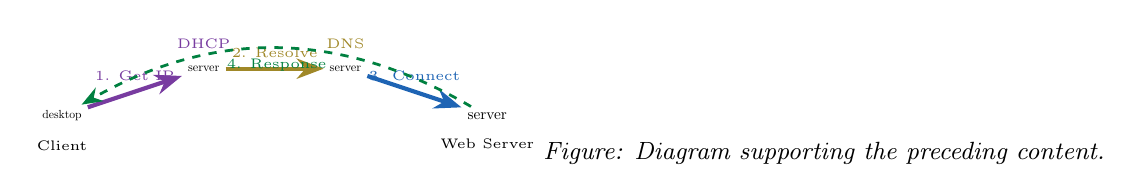
\begin{tikzpicture}[scale=0.6]
            % Client
            \node[pc] (client) at (0,0) {\iconpc[0.5cm]};
            \node[font=\tiny, below=0.05cm of client] {Client};
            
            % DHCP Server
            \node[server] (dhcp) at (3,1) {\iconserver[0.4cm]};
            \node[font=\tiny, dhcppurple, above=0.02cm of dhcp] {DHCP};
            
            % DNS Server
            \node[server] (dns) at (6,1) {\iconserver[0.4cm]};
            \node[font=\tiny, dnsyellow!80!black, above=0.02cm of dns] {DNS};
            
            % Web Server
            \node[server] (web) at (9,0) {\iconserver[0.5cm]};
            \node[font=\tiny, below=0.05cm of web] {Web Server};
            
            % Service chain arrows
            \draw[-{Stealth}, dhcppurple, line width=1.5pt] (client) -- (dhcp) 
                node[midway, above, font=\tiny] {1. Get IP};
            \draw[-{Stealth}, dnsyellow!80!black, line width=1.5pt] (dhcp) -- (dns) 
                node[midway, above, font=\tiny] {2. Resolve};
            \draw[-{Stealth}, tcpblue, line width=1.5pt] (dns) -- (web) 
                node[midway, above, font=\tiny] {3. Connect};
            
            % Return path
            \draw[-{Stealth}, networkgreen, line width=1pt, dashed] (web) to[bend right=30] 
                node[midway, below, font=\tiny] {4. Response} (client);
        \end{tikzpicture}
    \end{center}
\end{frame}

% Table of contents in presentation mode only
\presentationonly{
\begin{frame}[allowframebreaks]{Outline}
\small
\tableofcontents[hideallsubsections]
\end{frame}
}


% =============================================================================
% SLIDE 2: Review - Connecting to Module 5
% =============================================================================
\section*{Review from Module 5}

\begin{frame}{Review: Building on Module 5}
    \begin{columns}[T]
        \begin{column}{0.48\textwidth}
            \begin{block}{What We Learned (Module 5)}
                \small
                \begin{itemize}\setlength{\itemsep}{2pt}
                    \item \textbf{Routing}: How packets find their way
                    \item \textbf{NAT/PAT}: Address translation
                    \item \textbf{VLANs}: Network segmentation
                    \item \textbf{Firewalls}: Traffic filtering
                \end{itemize}
            \end{block}
            
            \vspace{0.3em}
            \begin{alertblock}{The Missing Piece}
                \small
                We can route packets, but how do devices \textbf{get their addresses}? How do they \textbf{find services} by name?
            \end{alertblock}
        \end{column}
        \begin{column}{0.48\textwidth}
            \begin{center}
    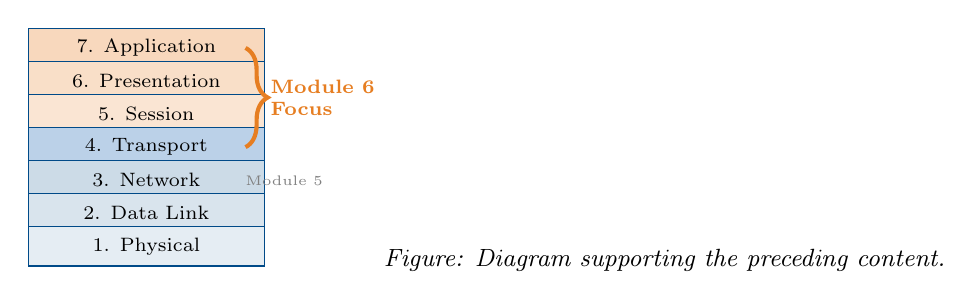
\begin{tikzpicture}[scale=0.7]
        % OSI layers - highlight 4-7
        \foreach \i/\name/\col in {
            7/Application/aborange!30,
            6/Presentation/aborange!25,
            5/Session/aborange!20,
            4/Transport/tcpblue!30,
            3/Network/rctcblue!20,
            2/Data Link/rctcblue!15,
            1/Physical/rctcblue!10} {
            \node[draw=rctcblue, fill=\col, minimum width=3cm, minimum height=0.5cm,
                  font=\scriptsize] at (0,\i*0.6-0.6) {\i. \name};
        }
        
        % Bracket for this module
        \draw[decorate, decoration={brace, amplitude=8pt}, line width=1.5pt, aborange]
            (1.8,3.6) -- (1.8,1.8);
        \node[font=\scriptsize\bfseries, aborange, align=left] at (3.2,2.7) {Module 6\\Focus};
        
        % Label for Module 5
        \node[font=\tiny, gray] at (2.5,1.2) {Module 5};
    \end{tikzpicture}
\end{center}
            
            \begin{exampleblock}{Module 6 Focus}
                \small
                \textbf{Services} that make networks usable: TCP/UDP, DHCP, DNS
            \end{exampleblock}
        \end{column}
    \end{columns}
\end{frame}

% =============================================================================
% SLIDE 3: Module 6 Overview
% =============================================================================
\section*{Learning Outcomes}

\begin{frame}{Module 6 Overview}
    \begin{columns}[T]
        \begin{column}{0.48\textwidth}
            \begin{block}{Topics Covered}
                \small
                \begin{enumerate}\setlength{\itemsep}{3pt}
                    \item \textbf{Transport Protocols} \\
                          {\scriptsize TCP, UDP, ports, connections}
                    \item \textbf{DHCP} \\
                          {\scriptsize Automatic IP configuration}
                    \item \textbf{APIPA \& SLAAC} \\
                          {\scriptsize Fallback and IPv6 auto-config}
                    \item \textbf{DHCP Troubleshooting} \\
                          {\scriptsize Relay agents, common issues}
                    \item \textbf{DNS Fundamentals} \\
                          {\scriptsize Name resolution, records}
                    \item \textbf{DNS Troubleshooting} \\
                          {\scriptsize nslookup, dig, common problems}
                \end{enumerate}
            \end{block}
        \end{column}
        \begin{column}{0.48\textwidth}
            \begin{block}{Learning Outcomes}
                \small
                By the end of this module, you will be able to:
                \begin{itemize}\setlength{\itemsep}{2pt}
                    \item Explain TCP vs UDP and when to use each
                    \item Describe the DHCP DORA process
                    \item Configure DHCP scopes and options
                    \item Explain DNS hierarchy and record types
                    \item Use nslookup and dig for troubleshooting
                    \item Identify common service misconfigurations
                \end{itemize}
            \end{block}
            
            \vspace{0.2em}
            \begin{exampleblock}{Batman Universe}
                \small
                Case studies featuring Batman, Oracle, Batgirl, Alfred, Catwoman, and The Riddler!
            \end{exampleblock}
        \end{column}
    \end{columns}
\end{frame}

\begin{frame}[t,allowframebreaks]{Learning Outcomes}
    After completing this module, you will be able to:
    \vspace{0.5em}
    \begin{itemize}
        \item Explain the differences between \keyterm{TCP} (reliable, connection-oriented) and \keyterm{UDP} (fast, connectionless) and identify appropriate use cases for each protocol.
        \item Describe how \keyterm{ports} (0--65535) identify services and how \keyterm{sockets} (IP address + port) establish connections between applications.
        \item Configure and manage \keyterm{DHCP} servers, including defining \keyterm{scopes}, creating \keyterm{reservations}, and setting \keyterm{DHCP options} (gateway, DNS, lease time).
        \item Explain the \keyterm{DORA} process (Discover, Offer, Request, Acknowledge) used by DHCP clients to obtain IP addresses.
        \item Configure \keyterm{DHCP relay agents} to forward DHCP messages across subnets and troubleshoot common DHCP issues.
        \item Describe \keyterm{APIPA} (169.254.x.x/16) as a fallback mechanism when DHCP is unavailable and explain its limitations (link-local only).
        \item Explain IPv6 \keyterm{SLAAC} (Stateless Address Autoconfiguration) using Router Advertisements and \keyterm{DHCPv6} (stateful and stateless modes).
        \item Describe the \keyterm{DNS} hierarchy (Root, TLD, Domain, Host) and explain how DNS resolves domain names to IP addresses.
        \item Identify common DNS record types: \keyterm{A} (IPv4), \keyterm{AAAA} (IPv6), \keyterm{CNAME} (alias), \keyterm{MX} (mail server), \keyterm{PTR} (reverse lookup).
        \item Use DNS troubleshooting tools like \keyterm{nslookup} and \keyterm{dig} to query DNS records, diagnose resolution issues, and verify zone transfers.
    \end{itemize}
\end{frame}

% =============================================================================
% SLIDE 5: Transport Layer and Ports
% =============================================================================
\section{Transport Layer Services}
\subsection{Ports, TCP, and UDP}

\articleonly{
This section reviews transport-layer behavior, port roles, and protocol tradeoffs between reliable and low-latency communication.
}

\begin{frame}{Transport Layer and Ports}
    \begin{columns}[T]
        \begin{column}{0.48\textwidth}
            \begin{itemize}
                \item \keyterm{Layer 4} provides host-to-host communication.
                \item \keyterm{Ports} identify specific services/applications.
                \item Port range: \textbf{0--65535}
                \item A \keyterm{socket} = IP address + port number
            \end{itemize}
            
            \vspace{0.2em}
            \begin{exampleblock}{Example}
                \small
                Web server: \texttt{10.0.0.5:443}
            \end{exampleblock}
        \end{column}
    \end{columns}
\end{frame}

% =============================================================================
% SLIDE 6: TCP - Reliable Delivery
% =============================================================================
\begin{frame}{TCP: Reliable Delivery}
    \begin{columns}[T]
        \begin{column}{0.48\textwidth}
            \begin{itemize}
                \item \keyterm{Transmission Control Protocol}
                \item \textbf{Connection-oriented}: Establishes session first
                \item \textbf{Reliable}: Guarantees delivery
                \item \textbf{Ordered}: Packets arrive in sequence
                \item \textbf{Error-checked}: Detects corruption
                \item \textbf{Flow control}: Prevents overwhelming receiver
            \end{itemize}
            
            \vspace{0.2em}
            \begin{alertblock}{Trade-off}
                \small
                Reliability costs \textbf{speed} and \textbf{overhead}. TCP headers are 20+ bytes.
            \end{alertblock}
        \end{column}
        \begin{column}{0.48\textwidth}
            \begin{block}{TCP Header (20+ bytes)}
                \centering
                \footnotesize
                \setlength{\tabcolsep}{1pt}
                \begin{tabular}{|>{\columncolor{tcpblue!15}}c|>{\columncolor{tcpblue!15}}c|}
                    \hline
                    \textbf{Source Port} & \textbf{Dest Port} \\
                    \hline
                    \multicolumn{2}{|>{\columncolor{tcpblue!15}}c|}{\textbf{Sequence Number}} \\
                    \hline
                    \multicolumn{2}{|>{\columncolor{tcpblue!15}}c|}{\textbf{Acknowledgment Number}} \\
                    \hline
                    Offset | \colorbox{aborange!30}{\textbf{Flags}} & Window Size \\
                    \hline
                    Checksum & Urgent Pointer \\
                    \hline
                    \multicolumn{2}{|>{\columncolor{tcpblue!5}}c|}{Options (variable)} \\
                    \hline
                \end{tabular}
                
                \vspace{0.3em}
                \scriptsize
                \colorbox{aborange!30}{Flags}: SYN, ACK, FIN, RST, PSH, URG
            \end{block}
            
            \vspace{0.2em}
            \begin{block}{Common TCP Applications}
                \small
                HTTP/S, FTP, SSH, SMTP, Telnet
            \end{block}
        \end{column}
    \end{columns}
\end{frame}

% =============================================================================
% SLIDE 7: TCP Three-Way Handshake (DIAGRAM)
% =============================================================================
\begin{frame}{TCP Three-Way Handshake}
    \begin{center}
        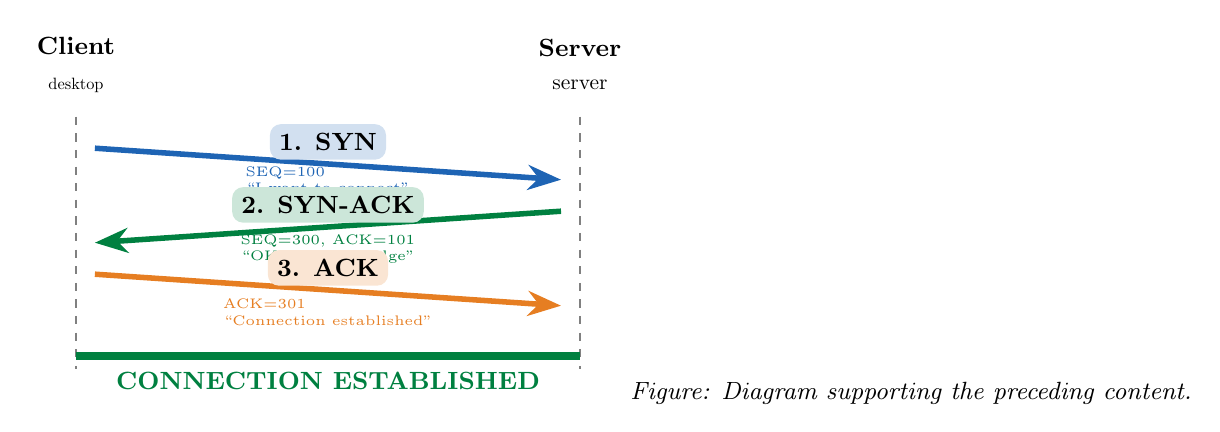
\begin{tikzpicture}[scale=0.8]
            % Client and Server
            \node[pc] (client) at (0,4) {\iconpc[0.7cm]};
            \node[font=\small\bfseries, above=0.1cm of client] {Client};
            
            \node[server] (server) at (8,4) {\iconserver[0.7cm]};
            \node[font=\small\bfseries, above=0.1cm of server] {Server};
            
            % Vertical timeline
            \draw[gray, line width=1pt, dashed] (0,3.5) -- (0,-0.5);
            \draw[gray, line width=1pt, dashed] (8,3.5) -- (8,-0.5);
            
            % Step 1: SYN
            \draw[-{Stealth}, tcpblue, line width=2pt] (0.3,3) -- (7.7,2.5);
            \node[fill=tcpblue!20, rounded corners, font=\small\bfseries] at (4,3.1) {1. SYN};
            \node[font=\tiny, tcpblue, align=left] at (4,2.5) {SEQ=100\\``I want to connect''};
            
            % Step 2: SYN-ACK
            \draw[-{Stealth}, networkgreen, line width=2pt] (7.7,2) -- (0.3,1.5);
            \node[fill=networkgreen!20, rounded corners, font=\small\bfseries] at (4,2.1) {2. SYN-ACK};
            \node[font=\tiny, networkgreen, align=left] at (4,1.4) {SEQ=300, ACK=101\\``OK, I acknowledge''};
            
            % Step 3: ACK
            \draw[-{Stealth}, aborange, line width=2pt] (0.3,1) -- (7.7,0.5);
            \node[fill=aborange!20, rounded corners, font=\small\bfseries] at (4,1.1) {3. ACK};
            \node[font=\tiny, aborange, align=left] at (4,0.4) {ACK=301\\``Connection established''};
            
            % Connection established indicator
            \draw[networkgreen, line width=3pt] (0,-0.3) -- (8,-0.3);
            \node[font=\small\bfseries, networkgreen] at (4,-0.7) {CONNECTION ESTABLISHED};
        \end{tikzpicture}
    \end{center}
    
    \vspace{0.3em}
    \begin{columns}[T]
        \begin{column}{0.48\textwidth}
            \begin{block}{Purpose}
                \small
                Synchronize sequence numbers and confirm both sides are ready to communicate.
            \end{block}
        \end{column}
        \begin{column}{0.48\textwidth}
            \begin{exampleblock}{Memory Tip}
                \small
                Think: ``\textbf{S}end $\rightarrow$ \textbf{S}end back with \textbf{A}ck $\rightarrow$ \textbf{A}cknowledge''
            \end{exampleblock}
        \end{column}
    \end{columns}
\end{frame}

% =============================================================================
% SLIDE 8: TCP Connection Teardown
% =============================================================================
\begin{frame}{TCP Connection Teardown}
    \begin{columns}[T]
        \begin{column}{0.45\textwidth}
            \begin{block}{Graceful Close (4-way)}
                \small
                \begin{enumerate}\setlength{\itemsep}{1pt}
                    \item \textbf{FIN}: ``I'm done sending''
                    \item \textbf{ACK}: ``Got it''
                    \item \textbf{FIN}: ``I'm done too''
                    \item \textbf{ACK}: ``Goodbye''
                \end{enumerate}
            \end{block}
            
            \vspace{0.2em}
            \begin{alertblock}{Abrupt Close (RST)}
                \small
                \textbf{RST} flag immediately terminates. Used when something goes wrong.
            \end{alertblock}
            
            \vspace{0.2em}
            \begin{exampleblock}{TIME\_WAIT}
                \small
                Socket waits ~2 min before reuse to avoid confusion with late packets.
            \end{exampleblock}
        \end{column}
        \begin{column}{0.52\textwidth}
            \begin{center}
                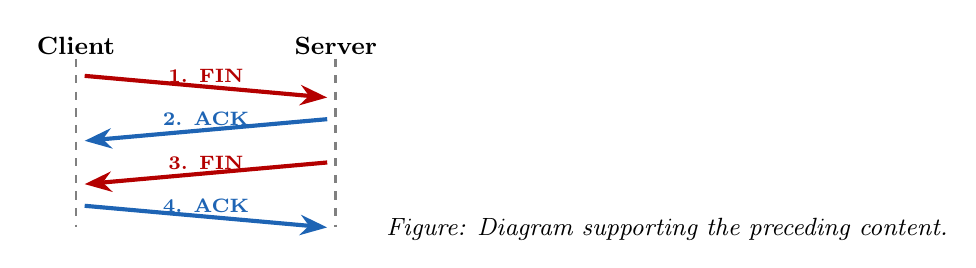
\begin{tikzpicture}[scale=0.55]
                    % Client and Server
                    \node[font=\small\bfseries] at (0,4.2) {Client};
                    \node[font=\small\bfseries] at (6,4.2) {Server};
                    
                    % Vertical timeline
                    \draw[gray, line width=1pt, dashed] (0,3.9) -- (0,0);
                    \draw[gray, line width=1pt, dashed] (6,3.9) -- (6,0);
                    
                    % Step 1: FIN
                    \draw[-{Stealth}, alertred, line width=1.5pt] (0.2,3.5) -- (5.8,3);
                    \node[font=\scriptsize\bfseries, alertred] at (3,3.5) {1. FIN};
                    
                    % Step 2: ACK
                    \draw[-{Stealth}, tcpblue, line width=1.5pt] (5.8,2.5) -- (0.2,2);
                    \node[font=\scriptsize\bfseries, tcpblue] at (3,2.5) {2. ACK};
                    
                    % Step 3: FIN
                    \draw[-{Stealth}, alertred, line width=1.5pt] (5.8,1.5) -- (0.2,1);
                    \node[font=\scriptsize\bfseries, alertred] at (3,1.5) {3. FIN};
                    
                    % Step 4: ACK
                    \draw[-{Stealth}, tcpblue, line width=1.5pt] (0.2,0.5) -- (5.8,0);
                    \node[font=\scriptsize\bfseries, tcpblue] at (3,0.5) {4. ACK};
                \end{tikzpicture}
            \end{center}
            
            \begin{block}{Key Point}
                \small
                Either side can initiate close. Process is bidirectional.
            \end{block}
        \end{column}
    \end{columns}
\end{frame}

% =============================================================================
% SLIDE 9: UDP - Fast and Simple
% =============================================================================
\begin{frame}{UDP: Fast and Simple}
    \begin{columns}[T]
        \begin{column}{0.48\textwidth}
            \begin{itemize}
                \item \keyterm{User Datagram Protocol}
                \item \textbf{Connectionless}: No handshake
                \item \textbf{Unreliable}: No delivery guarantee
                \item \textbf{Unordered}: May arrive out of order
                \item \textbf{No flow control}: Send as fast as possible
                \item ``Fire and forget''
            \end{itemize}
            
            \vspace{0.2em}
            \begin{exampleblock}{Why Use UDP?}
                \small
                When \textbf{speed} matters more than perfection: streaming, gaming, VoIP, DNS queries.
            \end{exampleblock}
            
            \vspace{0.2em}
            \begin{block}{Common UDP Applications}
                \small
                DNS, DHCP, TFTP, SNMP, VoIP, Streaming, Gaming
            \end{block}
        \end{column}
        \begin{column}{0.48\textwidth}
            \begin{block}{UDP Header (8 bytes only!)}
                \centering
                \small
                \setlength{\tabcolsep}{3pt}
                \begin{tabular}{|>{\columncolor{udpgreen!20}}c|>{\columncolor{udpgreen!20}}c|}
                    \hline
                    \textbf{Source Port} & \textbf{Dest Port} \\
                    16 bits & 16 bits \\
                    \hline
                    \textbf{Length} & \textbf{Checksum} \\
                    16 bits & 16 bits \\
                    \hline
                    \multicolumn{2}{|>{\columncolor{gray!10}}c|}{Data (Payload)} \\
                    \hline
                \end{tabular}
                
                \vspace{0.2em}
                \footnotesize
                \textcolor{udpgreen}{\textbf{Only 8 bytes}} vs TCP's 20+ bytes!
            \end{block}
            
            \vspace{0.3em}
            \begin{alertblock}{No Handshake Needed}
                \small
                Data sent immediately---no connection setup overhead. Trade-off: no delivery guarantee.
            \end{alertblock}
        \end{column}
    \end{columns}
\end{frame}

% =============================================================================
% SLIDE 10: TCP vs UDP Comparison
% =============================================================================
\begin{frame}{TCP vs UDP Comparison}
    \begin{center}
        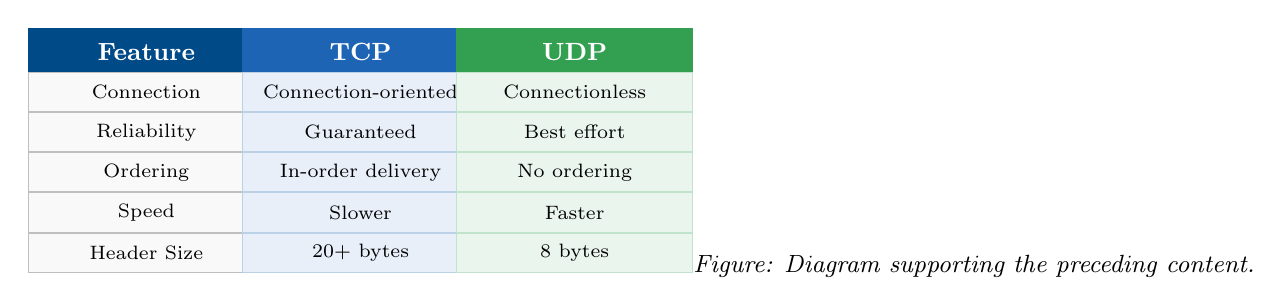
\begin{tikzpicture}[scale=0.85]
            % Table header
            \node[draw=rctcblue, fill=rctcblue, minimum width=3cm, minimum height=0.6cm,
                  font=\small\bfseries, text=white] at (0,3) {Feature};
            \node[draw=tcpblue, fill=tcpblue, minimum width=3cm, minimum height=0.6cm,
                  font=\small\bfseries, text=white] at (3.2,3) {TCP};
            \node[draw=udpgreen, fill=udpgreen, minimum width=3cm, minimum height=0.6cm,
                  font=\small\bfseries, text=white] at (6.4,3) {UDP};
            
            % Rows
            \foreach \y/\feature/\tcp/\udp in {
                2.4/Connection/Connection-oriented/Connectionless,
                1.8/Reliability/Guaranteed/Best effort,
                1.2/Ordering/In-order delivery/No ordering,
                0.6/Speed/Slower/Faster,
                0/Header Size/20+ bytes/8 bytes} {
                \node[draw=gray!50, fill=gray!5, minimum width=3cm, minimum height=0.5cm,
                      font=\scriptsize] at (0,\y) {\feature};
                \node[draw=tcpblue!30, fill=tcpblue!10, minimum width=3cm, minimum height=0.5cm,
                      font=\scriptsize] at (3.2,\y) {\tcp};
                \node[draw=udpgreen!30, fill=udpgreen!10, minimum width=3cm, minimum height=0.5cm,
                      font=\scriptsize] at (6.4,\y) {\udp};
            }
        \end{tikzpicture}
    \end{center}
    
    \vspace{0.3em}
    \begin{columns}[T]
        \begin{column}{0.48\textwidth}
            \begin{block}{Use TCP When...}
                \small
                \begin{itemize}\setlength{\itemsep}{1pt}
                    \item Data must arrive complete (files, email)
                    \item Order matters (web pages)
                    \item Errors are unacceptable (banking)
                \end{itemize}
            \end{block}
        \end{column}
        \begin{column}{0.48\textwidth}
            \begin{block}{Use UDP When...}
                \small
                \begin{itemize}\setlength{\itemsep}{1pt}
                    \item Speed is critical (gaming, video)
                    \item Small queries (DNS lookups)
                    \item Loss is tolerable (streaming)
                \end{itemize}
            \end{block}
        \end{column}
    \end{columns}
\end{frame}

% =============================================================================
% SLIDE 11: Case Study - Batman & Oracle
% =============================================================================
\begin{frame}{Case Study: Batman \& Oracle}
    \begin{casestudy}{The Mission Communications Problem}
        \small
        Batman is pursuing criminals through Gotham while coordinating with Oracle at the Clocktower. He needs to accomplish two things simultaneously:
        
        \vspace{0.3em}
        \begin{enumerate}\setlength{\itemsep}{2pt}
            \item Transfer surveillance footage from the Batmobile cameras to Oracle's servers (large video files, \textbf{must not lose any frames}).
            \item Maintain \textbf{real-time voice communication} with Oracle during the high-speed chase (some audio glitches are acceptable).
        \end{enumerate}
        
        \vspace{0.2em}
        The Batcomputer must choose the right transport protocol for each task.
    \end{casestudy}
    
    \begin{block}{Review Questions}
        \small
        \begin{enumerate}\setlength{\itemsep}{1pt}
            \item Which protocol should be used for the video file transfer? Why?
            \item Which protocol should be used for the voice communication? Why?
            \item What would happen if the protocols were swapped?
        \end{enumerate}
    \end{block}
\end{frame}

% =============================================================================
% SLIDE 12: Case Study Solution - Batman & Oracle
% =============================================================================
\begin{frame}{Case Study Solution: Batman \& Oracle}
    \begin{casesolution}{The Mission Communications Problem}
        \small
        \begin{enumerate}\setlength{\itemsep}{1pt}
            \item \textbf{Video files $\rightarrow$ TCP}: Missing frames corrupt evidence. TCP guarantees delivery.
            \item \textbf{Voice comms $\rightarrow$ UDP}: Real-time essential. Brief glitches beat lag. UDP wins.
            \item If swapped: Corrupted files (UDP) or unacceptable voice delay (TCP).
        \end{enumerate}
    \end{casesolution}
    
    \begin{center}
        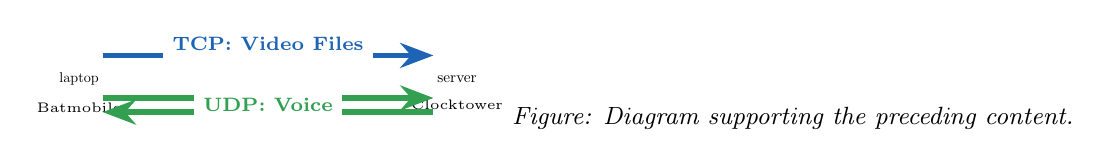
\begin{tikzpicture}[scale=0.6]
            % Batmobile
            \node[pc] (bat) at (0,0) {\iconlaptop[0.5cm]};
            \node[font=\tiny, below=0.02cm of bat] {Batmobile};
            
            % Clocktower
            \node[server] (oracle) at (8,0) {\iconserver[0.5cm]};
            \node[font=\tiny, below=0.02cm of oracle] {Clocktower};
            
            % TCP stream (files)
            \draw[-{Stealth}, tcpblue, line width=2pt] (0.5,0.5) -- (7.5,0.5);
            \node[font=\scriptsize\bfseries, tcpblue, fill=white] at (4,0.75) {TCP: Video Files};
            
            % UDP stream (voice)
            \draw[-{Stealth}, udpgreen, line width=2pt] (0.5,-0.4) -- (7.5,-0.4);
            \draw[{Stealth}-, udpgreen, line width=2pt] (0.5,-0.7) -- (7.5,-0.7);
            \node[font=\scriptsize\bfseries, udpgreen, fill=white] at (4,-0.55) {UDP: Voice};
        \end{tikzpicture}
    \end{center}
    
    \begin{alertblock}{Key Lesson}
        \small
        ``The mission requires choosing the right tool.'' Match protocol to need: reliability vs speed.
    \end{alertblock}
\end{frame}

% =============================================================================
% SLIDE 13: Common TCP and UDP Ports
% =============================================================================
\begin{frame}{Common TCP and UDP Ports}
    \begin{center}
        \small
        \begin{tabular}{c l l l}
            \toprule
            \textbf{Port} & \textbf{Protocol} & \textbf{Service} & \textbf{Description} \\
            \midrule
            \rowcolor{tcpblue!10} 20-21 & TCP & FTP & File Transfer Protocol \\
            \rowcolor{tcpblue!10} 22 & TCP & SSH & Secure Shell \\
            \rowcolor{tcpblue!10} 23 & TCP & Telnet & Remote terminal (insecure) \\
            \rowcolor{tcpblue!10} 25 & TCP & SMTP & Email sending \\
            \rowcolor{udpgreen!15} 53 & TCP/UDP & DNS & Domain Name System \\
            \rowcolor{udpgreen!10} 67-68 & UDP & DHCP & Dynamic Host Config \\
            \rowcolor{tcpblue!10} 80 & TCP & HTTP & Web (unencrypted) \\
            \rowcolor{tcpblue!10} 110 & TCP & POP3 & Email retrieval \\
            \rowcolor{tcpblue!10} 143 & TCP & IMAP & Email retrieval \\
            \rowcolor{tcpblue!10} 443 & TCP & HTTPS & Web (encrypted) \\
            \rowcolor{tcpblue!10} 3389 & TCP & RDP & Remote Desktop \\
            \bottomrule
        \end{tabular}
    \end{center}
    
    \vspace{0.3em}
    \begin{columns}[T]
        \begin{column}{0.48\textwidth}
            \begin{block}{Color Key}
                \small
                \colorbox{tcpblue!10}{TCP} \quad \colorbox{udpgreen!10}{UDP} \quad \colorbox{udpgreen!15}{Both}
            \end{block}
        \end{column}
        \begin{column}{0.48\textwidth}
            \begin{alertblock}{Exam Tip}
                \small
                Memorize these ports! They appear frequently on the Network+ exam.
            \end{alertblock}
        \end{column}
    \end{columns}
\end{frame}

% =============================================================================
% SLIDE 14: The netstat Command
% =============================================================================
\begin{frame}{The netstat Command}
    \begin{columns}[T]
        \begin{column}{0.48\textwidth}
            \begin{block}{What is netstat?}
                \small
                \keyterm{netstat} displays active connections, listening ports, and network statistics.
            \end{block}
            
            \vspace{0.2em}
            \begin{block}{Common Options}
                \footnotesize
                \begin{tabular}{l l}
                    \texttt{-a} & Show all connections \\
                    \texttt{-n} & Numeric (no DNS) \\
                    \texttt{-t/-u} & TCP/UDP only \\
                    \texttt{-l} & Listening ports only \\
                    \texttt{-p} & Show process ID \\
                \end{tabular}
            \end{block}
            
            \vspace{0.2em}
            \begin{alertblock}{Security Use}
                \small
                Identify suspicious connections or unexpected services.
            \end{alertblock}
        \end{column}
        \begin{column}{0.48\textwidth}
            \begin{block}{Sample Output}
                \ttfamily\tiny
                \begin{tabular}{l l l l}
                    Proto & Local & Foreign & State \\
                    \hline
                    tcp & 0.0.0.0:22 & *:* & LISTEN \\
                    tcp & 0.0.0.0:80 & *:* & LISTEN \\
                    tcp & 10.0.0.5:443 & 52.1.2.3:54321 & ESTAB \\
                    udp & 0.0.0.0:53 & *:* & \\
                \end{tabular}
            \end{block}
            
            \vspace{0.2em}
            \begin{exampleblock}{Reading Output}
                \small
                \begin{itemize}\setlength{\itemsep}{1pt}
                    \item \textbf{LISTEN}: Waiting for connections
                    \item \textbf{ESTABLISHED}: Active session
                    \item \textbf{0.0.0.0}: All interfaces
                \end{itemize}
            \end{exampleblock}
        \end{column}
    \end{columns}
\end{frame}

% =============================================================================
% SLIDE 15: DHCP Overview
% =============================================================================
\section{DHCP Address Management}
\subsection{DORA and Scope Configuration}

\articleonly{
DHCP automates IPv4 addressing and options distribution; this section covers leasing flow, scope design, and relay operation.
}

\begin{frame}{DHCP Overview}
    \begin{columns}[T]
        \begin{column}{0.48\textwidth}
            \begin{block}{The Problem}
                \small
                Manually configuring IP addresses on every device doesn't scale. Imagine a network with 500 devices!
            \end{block}
            
            \vspace{0.2em}
            \begin{block}{The Solution: DHCP}
                \small
                \keyterm{Dynamic Host Configuration Protocol} automatically assigns:
                \begin{itemize}\setlength{\itemsep}{1pt}
                    \item IP address
                    \item Subnet mask
                    \item Default gateway
                    \item DNS server addresses
                \end{itemize}
            \end{block}
           
        \end{column}
        \begin{column}{0.48\textwidth}
             \begin{alertblock}{Key Details}
                \small
                Uses \textbf{UDP ports 67} (server) and \textbf{68} (client). Client-server model with lease-based addressing.
            \end{alertblock}

            \begin{center}
                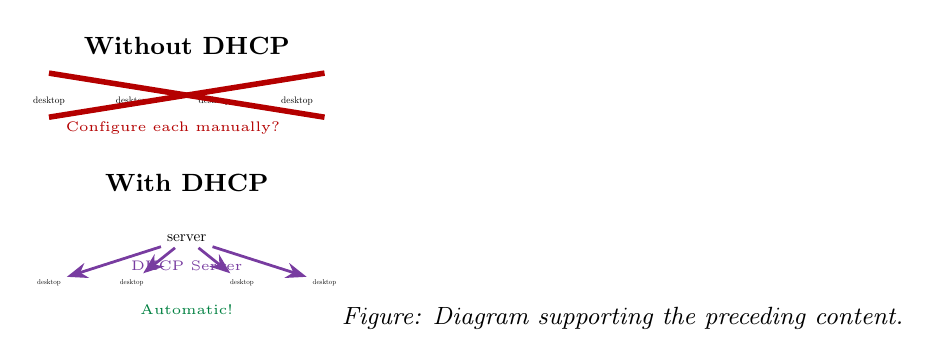
\begin{tikzpicture}[scale=0.7]
                    % Manual config (crossed out)
                    \node[font=\small\bfseries] at (2.5,3.5) {Without DHCP};
                    \node[pc] at (0,2.5) {\iconpc[0.4cm]};
                    \node[pc] at (1.5,2.5) {\iconpc[0.4cm]};
                    \node[pc] at (3,2.5) {\iconpc[0.4cm]};
                    \node[pc] at (4.5,2.5) {\iconpc[0.4cm]};
                    \node[font=\tiny, alertred] at (2.25,2) {Configure each manually?};
                    \draw[alertred, line width=2pt] (0,2.2) -- (5,3);
                    \draw[alertred, line width=2pt] (0,3) -- (5,2.2);
                    
                    % DHCP config
                    \node[font=\small\bfseries] at (2.5,1) {With DHCP};
                    \node[server] (dhcp) at (2.5,0) {\iconserver[0.5cm]};
                    \node[font=\tiny, dhcppurple] at (2.5,-0.5) {DHCP Server};
                    
                    \node[pc] (p1) at (0,-0.8) {\iconpc[0.3cm]};
                    \node[pc] (p2) at (1.5,-0.8) {\iconpc[0.3cm]};
                    \node[pc] (p3) at (3.5,-0.8) {\iconpc[0.3cm]};
                    \node[pc] (p4) at (5,-0.8) {\iconpc[0.3cm]};
                    
                    \draw[-{Stealth}, dhcppurple, line width=1pt] (dhcp) -- (p1);
                    \draw[-{Stealth}, dhcppurple, line width=1pt] (dhcp) -- (p2);
                    \draw[-{Stealth}, dhcppurple, line width=1pt] (dhcp) -- (p3);
                    \draw[-{Stealth}, dhcppurple, line width=1pt] (dhcp) -- (p4);
                    
                    \node[font=\tiny, networkgreen] at (2.5,-1.3) {Automatic!};
                \end{tikzpicture}
            \end{center}
        \end{column}
    \end{columns}
\end{frame}

% =============================================================================
% SLIDE 16: DHCP DORA Process (DIAGRAM)
% =============================================================================
\begin{frame}{DHCP DORA Process}
    \begin{center}
        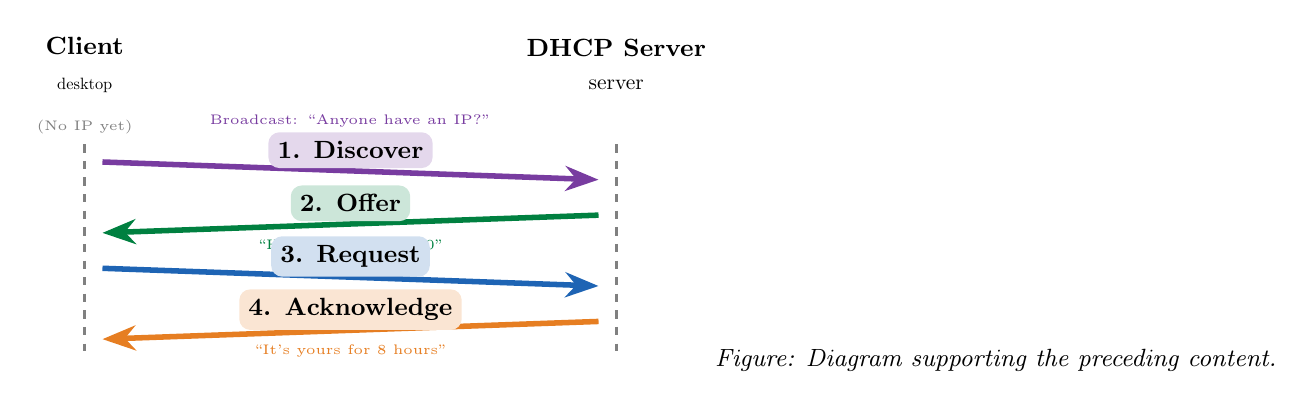
\begin{tikzpicture}[scale=0.75]
            % Client and Server
            \node[pc] (client) at (0,4) {\iconpc[0.7cm]};
            \node[font=\small\bfseries, above=0.1cm of client] {Client};
            \node[font=\tiny, gray] at (0,3.3) {(No IP yet)};
            
            \node[server] (server) at (9,4) {\iconserver[0.7cm]};
            \node[font=\small\bfseries, above=0.1cm of server] {DHCP Server};
            
            % Vertical timeline
            \draw[gray, line width=1pt, dashed] (0,3) -- (0,-0.5);
            \draw[gray, line width=1pt, dashed] (9,3) -- (9,-0.5);
            
            % D - Discover (broadcast)
            \draw[-{Stealth}, dhcppurple, line width=2pt] (0.3,2.7) -- (8.7,2.4);
            \node[fill=dhcppurple!20, rounded corners, font=\small\bfseries] at (4.5,2.9) {1. \textbf{D}iscover};
            \node[font=\tiny, dhcppurple] at (4.5,3.4) {Broadcast: ``Anyone have an IP?''};
            
            % O - Offer
            \draw[-{Stealth}, networkgreen, line width=2pt] (8.7,1.8) -- (0.3,1.5);
            \node[fill=networkgreen!20, rounded corners, font=\small\bfseries] at (4.5,2) {2. \textbf{O}ffer};
            \node[font=\tiny, networkgreen] at (4.5,1.3) {``Here's 192.168.1.100''};
            
            % R - Request
            \draw[-{Stealth}, tcpblue, line width=2pt] (0.3,0.9) -- (8.7,0.6);
            \node[fill=tcpblue!20, rounded corners, font=\small\bfseries] at (4.5,1.1) {3. \textbf{R}equest};
            \node[font=\tiny, tcpblue] at (4.5,0.4) {``I'll take that one!''};
            
            % A - Acknowledge
            \draw[-{Stealth}, aborange, line width=2pt] (8.7,0) -- (0.3,-0.3);
            \node[fill=aborange!20, rounded corners, font=\small\bfseries] at (4.5,0.2) {4. \textbf{A}cknowledge};
            \node[font=\tiny, aborange] at (4.5,-0.5) {``It's yours for 8 hours''};
        \end{tikzpicture}
    \end{center}
    
    \vspace{0.2em}
    \begin{columns}[T]
        \begin{column}{0.48\textwidth}
            \begin{block}{Memory Trick}
                \small
                \textbf{DORA} the Explorer finds IP addresses!
            \end{block}
        \end{column}
        \begin{column}{0.48\textwidth}
            \begin{exampleblock}{Lease Time}
                \small
                IP is ``rented'' for a set period. Client must renew before expiration.
            \end{exampleblock}
        \end{column}
    \end{columns}
\end{frame}

% =============================================================================
% SLIDE 17: DHCP Server Configuration
% =============================================================================
\begin{frame}{DHCP Server Configuration}
    \begin{columns}[T]
        \begin{column}{0.48\textwidth}
            \begin{block}{Scope (Address Pool)}
                \small
                A \keyterm{scope} defines the range of IP addresses the DHCP server can assign.
                
                \vspace{0.2em}
                \begin{tabular}{l l}
                    \textbf{Start IP} & 192.168.1.100 \\
                    \textbf{End IP} & 192.168.1.200 \\
                    \textbf{Subnet} & 255.255.255.0 \\
                    \textbf{Available} & 101 addresses \\
                \end{tabular}
            \end{block}
            
            \vspace{0.2em}
            \begin{block}{Lease Duration}
                \small
                \begin{itemize}\setlength{\itemsep}{1pt}
                    \item Typical: 8 hours to 8 days
                    \item Short leases: Mobile environments
                    \item Long leases: Stable networks
                    \item Client renews at 50\% of lease time
                \end{itemize}
            \end{block}
        \end{column}
        \begin{column}{0.48\textwidth}
            \begin{block}{Required Settings}
                \small
                \begin{itemize}\setlength{\itemsep}{2pt}
                    \item \textbf{IP range}: Start and end addresses
                    \item \textbf{Subnet mask}: Network size
                    \item \textbf{Default gateway}: Router IP
                    \item \textbf{DNS servers}: Name resolution
                    \item \textbf{Lease time}: How long to keep IP
                \end{itemize}
            \end{block}
            
            \vspace{0.2em}
            \begin{alertblock}{Best Practice}
                \small
                Leave some addresses outside the scope for static assignments (servers, printers, routers).
            \end{alertblock}
        \end{column}
    \end{columns}
\end{frame}

% =============================================================================
% SLIDE 18: DHCP Options
% =============================================================================
\begin{frame}{DHCP Options}
    \begin{columns}[T]
        \begin{column}{0.55\textwidth}
            \begin{block}{Common DHCP Options}
                \small
                \begin{tabular}{c l l}
                    \toprule
                    \textbf{Option} & \textbf{Name} & \textbf{Purpose} \\
                    \midrule
                    1 & Subnet Mask & Network size \\
                    3 & Default Gateway & Router address \\
                    6 & DNS Servers & Name resolution \\
                    15 & Domain Name & DNS suffix \\
                    51 & Lease Time & Duration in seconds \\
                    66 & TFTP Server & Boot server \\
                    150 & VoIP Server & Phone config \\
                    \bottomrule
                \end{tabular}
            \end{block}
            
            \vspace{0.2em}
            \begin{exampleblock}{Vendor Options}
                \small
                Options 43 and 60 allow vendor-specific settings for specialized devices.
            \end{exampleblock}
        \end{column}
        \begin{column}{0.42\textwidth}
            \begin{block}{How Options Work}
                \small
                DHCP options are sent with the Offer and Acknowledge messages.
                
                \vspace{0.2em}
                Client receives:
                \begin{itemize}\setlength{\itemsep}{1pt}
                    \item IP: 192.168.1.100
                    \item Mask: 255.255.255.0
                    \item Gateway: 192.168.1.1
                    \item DNS: 8.8.8.8
                \end{itemize}
            \end{block}
            
            \vspace{0.2em}
            \begin{alertblock}{NTP Option}
                \small
                Option 42 provides time servers---critical for authentication!
            \end{alertblock}
        \end{column}
    \end{columns}
\end{frame}

% =============================================================================
% SLIDE 19: DHCP Reservations and Exclusions
% =============================================================================
\begin{frame}{DHCP Reservations and Exclusions}
    \begin{columns}[T]
        \begin{column}{0.48\textwidth}
            \begin{block}{Reservations}
                \small
                A \keyterm{reservation} binds a specific IP to a MAC address. The device always gets the same IP.
                
                \vspace{0.2em}
                \textbf{Use for:}
                \begin{itemize}\setlength{\itemsep}{1pt}
                    \item Servers
                    \item Network printers
                    \item Security cameras
                    \item VoIP phones
                \end{itemize}
            \end{block}
            
            \vspace{0.2em}
            \begin{exampleblock}{Reservation Example}
                \small
                MAC: \texttt{AA:BB:CC:11:22:33} \\
                Reserved IP: \texttt{192.168.1.50}
            \end{exampleblock}
        \end{column}
        \begin{column}{0.48\textwidth}
            \begin{block}{Exclusions}
                \small
                An \keyterm{exclusion} removes addresses from the DHCP pool. These IPs will never be assigned.
                
                \vspace{0.2em}
                \textbf{Use for:}
                \begin{itemize}\setlength{\itemsep}{1pt}
                    \item Statically configured devices
                    \item Router interfaces
                    \item Addresses already in use
                \end{itemize}
            \end{block}
            
            \vspace{0.2em}
            \begin{alertblock}{Key Difference}
                \small
                \textbf{Reservation}: DHCP assigns specific IP to specific MAC. \\
                \textbf{Exclusion}: DHCP never touches these IPs.
            \end{alertblock}
        \end{column}
    \end{columns}
\end{frame}

% =============================================================================
% SLIDE 20: DHCP Relay and IP Helper (DIAGRAM)
% =============================================================================
\begin{frame}{DHCP Relay and IP Helper}
    \begin{columns}[T]
        \begin{column}{0.42\textwidth}
            \begin{block}{The Problem}
                \small
                DHCP Discover is a \textbf{broadcast}. Broadcasts don't cross routers! How do remote subnets get DHCP?
            \end{block}
            
            \vspace{0.2em}
            \begin{block}{The Solution}
                \small
                \keyterm{DHCP Relay} (IP Helper) forwards DHCP broadcasts to a remote server as unicast.
                
                \vspace{0.2em}
                \texttt{ip helper-address 10.0.0.5}
            \end{block}
            
            \vspace{0.2em}
            \begin{alertblock}{Configure On}
                \small
                The router interface facing the clients (not the server).
            \end{alertblock}
        \end{column}
        \begin{column}{0.55\textwidth}
            \begin{center}
                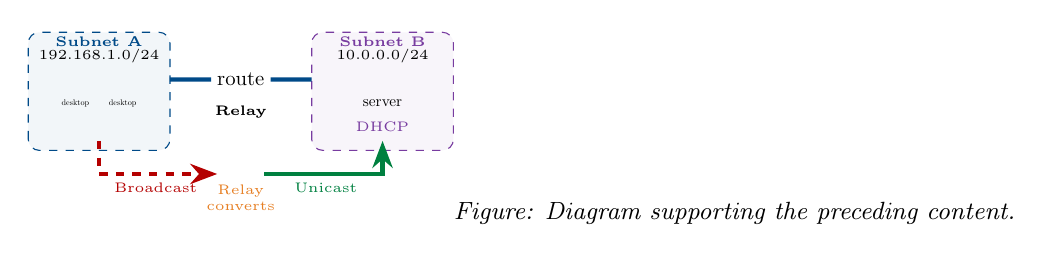
\begin{tikzpicture}[scale=0.6]
                    % Subnet A (clients)
                    \draw[dashed, rctcblue, rounded corners, fill=rctcblue!5] 
                        (-0.5,-0.5) rectangle (2.5,2);
                    \node[font=\tiny\bfseries, rctcblue] at (1,1.8) {Subnet A};
                    \node[font=\tiny] at (1,1.5) {192.168.1.0/24};
                    
                    \node[pc] (pc1) at (0.5,0.5) {\iconpc[0.35cm]};
                    \node[pc] (pc2) at (1.5,0.5) {\iconpc[0.35cm]};
                    
                    % Router with relay
                    \node[router] (rtr) at (4,1) {\iconrouter[0.6cm]};
                    \node[font=\tiny\bfseries, below=0.05cm of rtr] {Relay};
                    
                    % Subnet B (DHCP server)
                    \draw[dashed, dhcppurple, rounded corners, fill=dhcppurple!5] 
                        (5.5,-0.5) rectangle (8.5,2);
                    \node[font=\tiny\bfseries, dhcppurple] at (7,1.8) {Subnet B};
                    \node[font=\tiny] at (7,1.5) {10.0.0.0/24};
                    
                    \node[server] (dhcp) at (7,0.5) {\iconserver[0.5cm]};
                    \node[font=\tiny, dhcppurple] at (7,0) {DHCP};
                    
                    % Connections
                    \draw[ethernet noarrow] (2.5,1) -- (rtr);
                    \draw[ethernet noarrow] (rtr) -- (5.5,1);
                    
                    % Broadcast arrow
                    \draw[-{Stealth}, alertred, line width=1.5pt, dashed] 
                        (1,-0.3) -- (1,-1) -- (3.5,-1);
                    \node[font=\tiny, alertred] at (2.2,-1.3) {Broadcast};
                    
                    % Unicast arrow
                    \draw[-{Stealth}, networkgreen, line width=1.5pt] 
                        (4.5,-1) -- (7,-1) -- (7,-0.3);
                    \node[font=\tiny, networkgreen] at (5.8,-1.3) {Unicast};
                    
                    % Relay conversion
                    \node[font=\tiny, aborange, align=center] at (4,-1.5) {Relay\\converts};
                \end{tikzpicture}
            \end{center}
            
            \vspace{0.2em}
            \begin{exampleblock}{Result}
                \small
                One DHCP server can serve multiple subnets through relay agents.
            \end{exampleblock}
        \end{column}
    \end{columns}
\end{frame}

% =============================================================================
% SLIDE 21: Case Study - Batgirl & Alfred
% =============================================================================
\begin{frame}{Case Study: Batgirl \& Alfred}
    \begin{casestudy}{The Wayne Manor Network Problem}
        \small
        Batgirl installed new training equipment in the Wayne Manor gym (\textbf{VLAN 30}). All devices are getting \texttt{169.254.x.x} addresses! The DHCP server is on \textbf{VLAN 10} and works fine there.
        
        \vspace{0.2em}
        \footnotesize
        \begin{center}
            \begin{tabular}{l l l}
                \toprule
                \textbf{VLAN} & \textbf{Subnet} & \textbf{Purpose} \\
                \midrule
                VLAN 10 & 192.168.10.0/24 & Main house (DHCP here) \\
                VLAN 30 & 192.168.30.0/24 & Gym (problem devices) \\
                \bottomrule
            \end{tabular}
        \end{center}
    \end{casestudy}
    
    \begin{block}{Review Questions}
        \small
        \begin{enumerate}\setlength{\itemsep}{1pt}
            \item What does the 169.254.x.x address indicate?
            \item Why can't devices on VLAN 30 reach the DHCP server?
            \item What solution would fix this problem?
        \end{enumerate}
    \end{block}
\end{frame}

% =============================================================================
% SLIDE 22: Case Study Solution - Batgirl & Alfred
% =============================================================================
\begin{frame}{Case Study Solution: Batgirl \& Alfred}
    \begin{casesolution}{The Wayne Manor Network Problem}
        \small
        \begin{enumerate}\setlength{\itemsep}{1pt}
            \item \textbf{169.254.x.x} = APIPA address. DHCP failed, device assigned link-local IP.
            \item \textbf{DHCP broadcasts don't cross VLANs/subnets}. The router blocks them.
            \item Configure \keyterm{DHCP Relay} on VLAN 30's router interface: \\
                  \texttt{ip helper-address 192.168.10.5}
        \end{enumerate}
    \end{casesolution}
    
    \begin{center}
        
\begin{tikzpicture}[scale=0.55]
            % VLAN 30 (Gym)
            \node[pc] (gym) at (0,0) {\iconpc[0.5cm]};
            \node[font=\tiny, below=0.02cm of gym] {Gym Equipment};
            \node[font=\tiny, rctcblue] at (0,0.7) {VLAN 30};
            
            % Router
            \node[router] (rtr) at (4,0) {\iconrouter[0.6cm]};
            \node[font=\tiny\bfseries, aborange, above=0.05cm of rtr] {ip helper-address};
            
            % DHCP Server (VLAN 10)
            \node[server] (dhcp) at (8,0) {\iconserver[0.5cm]};
            \node[font=\tiny, below=0.02cm of dhcp] {DHCP Server};
            \node[font=\tiny, dhcppurple] at (8,0.7) {VLAN 10};
            
            % Flow
            \draw[-{Stealth}, alertred, line width=1.5pt] (0.5,0) -- (3.3,0);
            \node[font=\tiny, alertred] at (1.9,0.3) {Broadcast};
            
            \draw[-{Stealth}, networkgreen, line width=1.5pt] (4.7,0) -- (7.3,0);
            \node[font=\tiny, networkgreen] at (6,0.3) {Unicast};
            
            \draw[-{Stealth}, networkgreen, line width=1.5pt, dashed] (7.3,-0.3) -- (0.5,-0.3);
            \node[font=\tiny, networkgreen] at (4,-0.6) {IP Assigned!};
        \end{tikzpicture}
    \end{center}
    
    \begin{alertblock}{Key Lesson}
        \small
        ``Even the Bat-family needs proper network configuration, Miss Barbara.'' --- Alfred. \\
        DHCP relay enables centralized DHCP across multiple subnets.
    \end{alertblock}
\end{frame}

% =============================================================================
% SLIDE 23: APIPA - Automatic Private IP Addressing
% =============================================================================
\begin{frame}{APIPA: Automatic Private IP Addressing}
    \begin{columns}[T]
        \begin{column}{0.48\textwidth}
            \begin{block}{What is APIPA?}
                \small
                When DHCP fails, devices assign themselves an IP from the \keyterm{169.254.0.0/16} range.
                
                \vspace{0.2em}
                \begin{itemize}\setlength{\itemsep}{1pt}
                    \item Automatic fallback mechanism
                    \item Link-local addresses only
                    \item No gateway, no DNS
                    \item Can only talk to local subnet
                \end{itemize}
            \end{block}
            
            \vspace{0.2em}
            \begin{alertblock}{Symptom Alert}
                \small
                If you see \texttt{169.254.x.x}, DHCP is broken! Check server, network path, or relay.
            \end{alertblock}
        \end{column}
        \begin{column}{0.48\textwidth}
            \begin{center}
                \begin{tikzpicture}[scale=0.7]
                    % Client trying DHCP
                    \node[pc] (pc) at (0,2) {\iconpc[0.5cm]};
                    \node[font=\tiny] at (0,1.4) {Client};
                    
                    % DHCP attempt (failed)
                    \draw[-{Stealth}, alertred, line width=1.5pt, dashed] (0.5,2) -- (3,2);
                    \node[font=\tiny, alertred] at (1.75,2.4) {DHCP Discover};
                    
                    % No response
                    \node[font=\scriptsize, alertred] at (4,2) {\faTimesCircle};
                    \node[font=\tiny, alertred] at (4,1.5) {No response};
                    
                    % APIPA assignment
                    \draw[-{Stealth}, aborange, line width=1.5pt] (0,1) -- (0,0);
                    \node[font=\tiny, aborange, align=center] at (1.8,0.5) {Self-assign\\APIPA};
                    
                    % Result
                    \node[draw=aborange, fill=aborange!10, rounded corners, 
                          font=\small\ttfamily] at (0,-0.5) {169.254.x.x};
                \end{tikzpicture}
            \end{center}
            
            \vspace{0.2em}
            \begin{exampleblock}{Limited Connectivity}
                \small
                APIPA devices can communicate with each other but cannot reach the internet or other subnets.
            \end{exampleblock}
        \end{column}
    \end{columns}
\end{frame}

% =============================================================================
% SLIDE 24: DHCP Troubleshooting
% =============================================================================
\begin{frame}{DHCP Troubleshooting}
    \begin{columns}[T]
        \begin{column}{0.48\textwidth}
            \begin{block}{Common DHCP Issues}
                \small
                \begin{itemize}\setlength{\itemsep}{2pt}
                    \item \textbf{Server down}: Service stopped
                    \item \textbf{Scope exhausted}: No IPs left
                    \item \textbf{Wrong VLAN}: Client isolated
                    \item \textbf{Firewall blocking}: Ports 67/68
                    \item \textbf{Rogue DHCP}: Unauthorized server
                    \item \textbf{Relay missing}: Cross-subnet issue
                \end{itemize}
            \end{block}
            
            \vspace{0.2em}
            \begin{alertblock}{Rogue DHCP}
                \small
                Unauthorized DHCP servers can give wrong IPs, gateways, or DNS---security risk!
            \end{alertblock}
        \end{column}
        \begin{column}{0.48\textwidth}
            \begin{block}{Troubleshooting Commands}
                \scriptsize
                \textbf{Windows:}
                \begin{itemize}\setlength{\itemsep}{1pt}
                    \item \texttt{ipconfig /release}
                    \item \texttt{ipconfig /renew}
                    \item \texttt{ipconfig /all}
                \end{itemize}
                
                \vspace{0.2em}
                \scriptsize
                \textbf{Linux:}
                \begin{itemize}\setlength{\itemsep}{1pt}
                    \item \texttt{dhclient -r} (release)
                    \item \texttt{dhclient} (renew)
                    \item \texttt{ip addr show}
                \end{itemize}
            \end{block}
            
            \vspace{0.2em}
            \begin{exampleblock}{Quick Check}
                \small
                Got 169.254.x.x? $\rightarrow$ DHCP failed \\
                Got 0.0.0.0? $\rightarrow$ No address assigned
            \end{exampleblock}
        \end{column}
    \end{columns}
\end{frame}

% =============================================================================
% SLIDE 25: IPv6 SLAAC
% =============================================================================
\section{IPv6 Address Assignment}
\subsection{SLAAC and DHCPv6}

\articleonly{
IPv6 hosts can self-configure through router advertisements or use DHCPv6 depending on deployment requirements and policy.
}

\begin{frame}{IPv6 SLAAC: Stateless Address Autoconfiguration}
    \begin{columns}[T]
        \begin{column}{0.48\textwidth}
            \begin{block}{What is SLAAC?}
                \small
                \keyterm{SLAAC} lets IPv6 hosts configure themselves \textbf{without a DHCP server}.
                
                \vspace{0.2em}
                \begin{enumerate}\setlength{\itemsep}{1pt}
                    \item Router sends \textbf{prefix} (RA)
                    \item Host generates \textbf{interface ID}
                    \item Combines: prefix + interface ID
                    \item Result: Full IPv6 address
                \end{enumerate}
            \end{block}
            
            \vspace{0.2em}
            \begin{block}{EUI-64}
                \small
                Interface ID created from MAC address:
                \begin{itemize}\setlength{\itemsep}{1pt}
                    \item Insert \texttt{FF:FE} in middle
                    \item Flip 7th bit
                \end{itemize}
            \end{block}
        \end{column}
        \begin{column}{0.48\textwidth}
            \begin{center}
                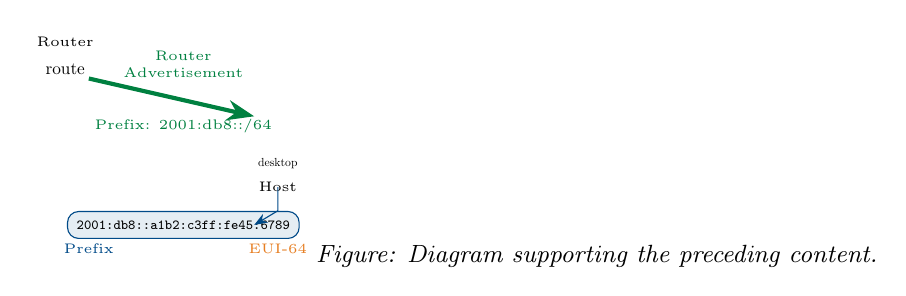
\begin{tikzpicture}[scale=0.6]
                    % Router
                    \node[router] (rtr) at (0,2.5) {\iconrouter[0.5cm]};
                    \node[font=\tiny, above=0.02cm of rtr] {Router};
                    
                    % RA message
                    \draw[-{Stealth}, networkgreen, line width=1.5pt] (0.5,2.3) -- (4,1.5);
                    \node[font=\tiny, networkgreen, align=center] at (2.5,2.6) {Router\\Advertisement};
                    \node[font=\tiny, networkgreen] at (2.5,1.3) {Prefix: 2001:db8::/64};
                    
                    % Host
                    \node[pc] (pc) at (4.5,0.5) {\iconpc[0.5cm]};
                    \node[font=\tiny] at (4.5,0) {Host};
                    
                    % Generated address
                    \node[draw=rctcblue, fill=rctcblue!10, rounded corners,
                          font=\tiny\ttfamily, align=center] at (2.5,-0.8) 
                          {2001:db8::a1b2:c3ff:fe45:6789};
                    \draw[-{Stealth}, rctcblue] (4.5,0) -- (4.5,-0.5) -- (4,-0.8);
                    
                    % Labels
                    \node[font=\tiny, rctcblue] at (0.5,-1.3) {Prefix};
                    \node[font=\tiny, aborange] at (4.5,-1.3) {EUI-64};
                \end{tikzpicture}
            \end{center}
            
            \vspace{0.3em}
            \begin{exampleblock}{No Server Needed}
                \small
                SLAAC is truly stateless---router just advertises prefix, host does the rest!
            \end{exampleblock}
        \end{column}
    \end{columns}
\end{frame}

% =============================================================================
% SLIDE 26: DHCPv6
% =============================================================================
\begin{frame}{DHCPv6: IPv6 Address Assignment}
    \begin{columns}[T]
        \begin{column}{0.48\textwidth}
            \begin{block}{DHCPv6 Modes}
                \small
                \textbf{Stateful DHCPv6:}
                \begin{itemize}\setlength{\itemsep}{1pt}
                    \item Server assigns full address
                    \item Tracks leases like DHCPv4
                    \item Full control over addressing
                \end{itemize}
                
                \vspace{0.2em}
                \textbf{Stateless DHCPv6:}
                \begin{itemize}\setlength{\itemsep}{1pt}
                    \item SLAAC provides address
                    \item DHCPv6 provides options only
                    \item DNS, NTP, domain name
                \end{itemize}
            \end{block}
        \end{column}
        \begin{column}{0.48\textwidth}
            \begin{block}{Router Advertisement Flags}
                \small
                \begin{tabular}{l l}
                    \textbf{M flag} & Managed (use DHCPv6) \\
                    \textbf{O flag} & Other (get options) \\
                \end{tabular}
                
                \vspace{0.3em}
                \footnotesize
                \begin{tabular}{c c l}
                    \textbf{M} & \textbf{O} & \textbf{Result} \\
                    \hline
                    0 & 0 & SLAAC only \\
                    0 & 1 & SLAAC + DHCPv6 options \\
                    1 & 0 & Stateful DHCPv6 \\
                    1 & 1 & Stateful + options \\
                \end{tabular}
            \end{block}
            
            \vspace{0.2em}
            \begin{alertblock}{Key Difference}
                \small
                DHCPv4 uses broadcast; DHCPv6 uses multicast (ff02::1:2).
            \end{alertblock}
        \end{column}
    \end{columns}
\end{frame}

% =============================================================================
% SLIDE 27: DNS - Why We Need It
% =============================================================================
\section{DNS Resolution Services}
\subsection{Hierarchy, Records, and Operations}

\articleonly{
This section covers DNS hierarchy, record types, recursion, and operational troubleshooting for name resolution services.
}

\begin{frame}{DNS: The Internet's Phone Book}
    \begin{columns}[T]
        \begin{column}{0.48\textwidth}
            \begin{block}{The Problem}
                \small
                Humans remember \textbf{names}, computers use \textbf{numbers}.
                
                \vspace{0.2em}
                Which is easier to remember?
                \begin{itemize}
                    \item \texttt{www.google.com}
                    \item \texttt{142.250.80.100}
                \end{itemize}
            \end{block}
            
            \vspace{0.2em}
            \begin{block}{The Solution: DNS}
                \small
                \keyterm{Domain Name System} translates names to IP addresses (and vice versa).
                
                \vspace{0.2em}
                \begin{itemize}\setlength{\itemsep}{1pt}
                    \item Uses \textbf{UDP port 53} (queries)
                    \item Uses \textbf{TCP port 53} (zone transfers)
                    \item Hierarchical, distributed database
                \end{itemize}
            \end{block}
        \end{column}
        \begin{column}{0.48\textwidth}
            \begin{center}
                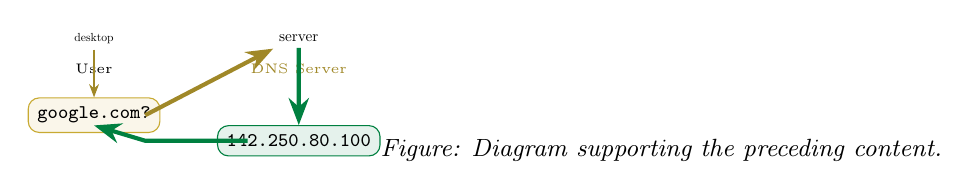
\begin{tikzpicture}[scale=0.65]
                    % User query
                    \node[pc] (user) at (0,2) {\iconpc[0.5cm]};
                    \node[font=\tiny] at (0,1.4) {User};
                    
                    % DNS query
                    \node[draw=dnsyellow, fill=dnsyellow!10, rounded corners,
                          font=\scriptsize\ttfamily] (query) at (0,0.5) {google.com?};
                    \draw[-{Stealth}, dnsyellow!80!black] (user) -- (query);
                    
                    % DNS Server
                    \node[server] (dns) at (4,2) {\iconserver[0.5cm]};
                    \node[font=\tiny, dnsyellow!80!black] at (4,1.4) {DNS Server};
                    
                    % Query arrow
                    \draw[-{Stealth}, dnsyellow!80!black, line width=1.5pt] (1,0.5) -- (3.5,1.8);
                    
                    % Response
                    \node[draw=networkgreen, fill=networkgreen!10, rounded corners,
                          font=\scriptsize\ttfamily] (resp) at (4,0) {142.250.80.100};
                    \draw[-{Stealth}, networkgreen, line width=1.5pt] (dns) -- (resp);
                    \draw[-{Stealth}, networkgreen, line width=1.5pt] (3,0) -- (1,0) -- (0,0.3);
                \end{tikzpicture}
            \end{center}
            
            \vspace{0.2em}
            \begin{exampleblock}{Critical Service}
                \small
                Without DNS, you'd need to memorize IP addresses for every website!
            \end{exampleblock}
        \end{column}
    \end{columns}
\end{frame}

% =============================================================================
% SLIDE 28: DNS Hierarchy (DIAGRAM)
% =============================================================================
\begin{frame}{DNS Hierarchy}
    \begin{center}
        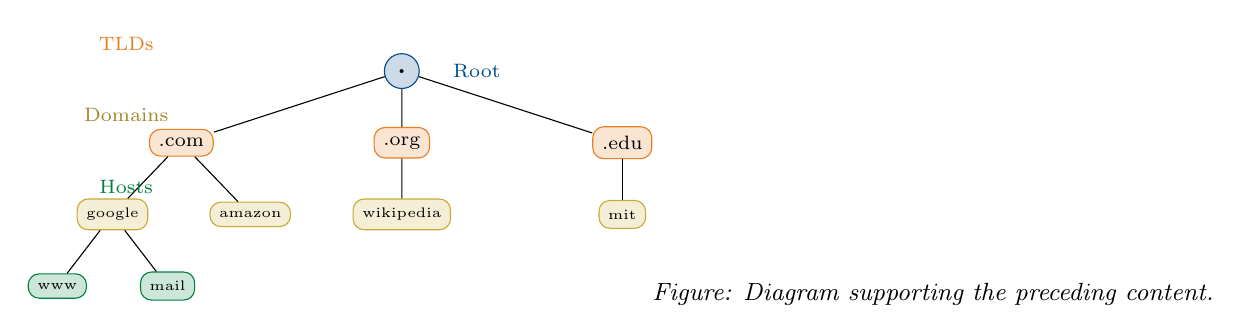
\begin{tikzpicture}[scale=0.7,
            level 1/.style={sibling distance=4cm, level distance=1.3cm},
            level 2/.style={sibling distance=2.5cm, level distance=1.3cm},
            level 3/.style={sibling distance=2cm, level distance=1.3cm}]
            
            % Root
            \node[draw=rctcblue, fill=rctcblue!20, circle, font=\small\bfseries] (root) {.}
                child {node[draw=aborange, fill=aborange!20, rounded corners, font=\scriptsize] {.com}
                    child {node[draw=dnsyellow, fill=dnsyellow!20, rounded corners, font=\tiny] {google}
                        child {node[draw=networkgreen, fill=networkgreen!20, rounded corners, font=\tiny] {www}}
                        child {node[draw=networkgreen, fill=networkgreen!20, rounded corners, font=\tiny] {mail}}
                    }
                    child {node[draw=dnsyellow, fill=dnsyellow!20, rounded corners, font=\tiny] {amazon}}
                }
                child {node[draw=aborange, fill=aborange!20, rounded corners, font=\scriptsize] {.org}
                    child {node[draw=dnsyellow, fill=dnsyellow!20, rounded corners, font=\tiny] {wikipedia}}
                }
                child {node[draw=aborange, fill=aborange!20, rounded corners, font=\scriptsize] {.edu}
                    child {node[draw=dnsyellow, fill=dnsyellow!20, rounded corners, font=\tiny] {mit}}
                };
            
            % Labels
            \node[font=\scriptsize, rctcblue, right=0.3cm of root] {Root};
            \node[font=\scriptsize, aborange] at (-5,0.5) {TLDs};
            \node[font=\scriptsize, dnsyellow!80!black] at (-5,-0.8) {Domains};
            \node[font=\scriptsize, networkgreen] at (-5,-2.1) {Hosts};
        \end{tikzpicture}
    \end{center}
    
    \vspace{0.2em}
    \begin{columns}[T]
        \begin{column}{0.48\textwidth}
            \begin{block}{FQDN Example}
                \small
                \texttt{www.google.com.} \\
                \footnotesize
                Host.Domain.TLD.Root
            \end{block}
        \end{column}
        \begin{column}{0.48\textwidth}
            \begin{exampleblock}{13 Root Servers}
                \small
                Named A through M, distributed globally with anycast.
            \end{exampleblock}
        \end{column}
    \end{columns}
\end{frame}

% =============================================================================
% SLIDE 29: DNS Name Resolution Process
% =============================================================================
\begin{frame}{DNS Name Resolution Process}
    \begin{center}
        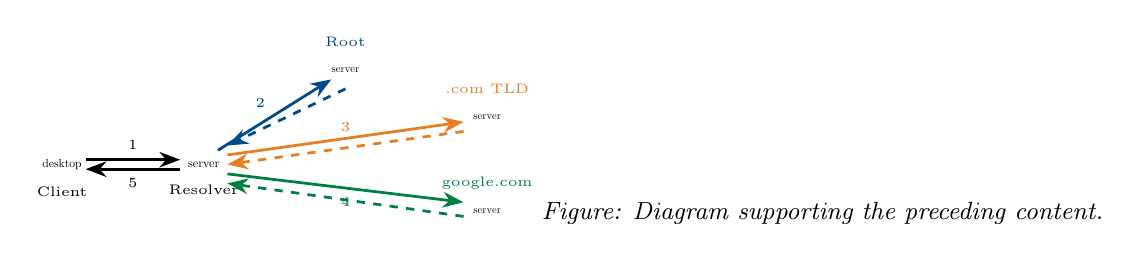
\begin{tikzpicture}[scale=0.6]
            % Client
            \node[pc] (client) at (0,0) {\iconpc[0.5cm]};
            \node[font=\tiny, below=0.02cm of client] {Client};
            
            % Recursive resolver
            \node[server] (resolver) at (3,0) {\iconserver[0.4cm]};
            \node[font=\tiny, below=0.02cm of resolver] {Resolver};
            
            % Root server
            \node[server] (root) at (6,2) {\iconserver[0.35cm]};
            \node[font=\tiny, rctcblue] at (6,2.6) {Root};
            
            % TLD server
            \node[server] (tld) at (9,1) {\iconserver[0.35cm]};
            \node[font=\tiny, aborange] at (9,1.6) {.com TLD};
            
            % Authoritative
            \node[server] (auth) at (9,-1) {\iconserver[0.35cm]};
            \node[font=\tiny, networkgreen] at (9,-0.4) {google.com};
            
            % Queries
            \draw[-{Stealth}, line width=1pt] (0.5,0.1) -- (2.5,0.1);
            \node[font=\tiny] at (1.5,0.4) {1};
            
            \draw[-{Stealth}, line width=1pt, rctcblue] (3.3,0.3) -- (5.7,1.8);
            \node[font=\tiny, rctcblue] at (4.2,1.3) {2};
            
            \draw[-{Stealth}, line width=1pt, rctcblue, dashed] (6,1.6) -- (3.5,0.4);
            
            \draw[-{Stealth}, line width=1pt, aborange] (3.5,0.2) -- (8.5,0.9);
            \node[font=\tiny, aborange] at (6,0.8) {3};
            
            \draw[-{Stealth}, line width=1pt, aborange, dashed] (8.5,0.7) -- (3.5,0);
            
            \draw[-{Stealth}, line width=1pt, networkgreen] (3.5,-0.2) -- (8.5,-0.8);
            \node[font=\tiny, networkgreen] at (6,-0.8) {4};
            
            \draw[-{Stealth}, line width=1pt, networkgreen, dashed] (8.5,-1.1) -- (3.5,-0.4);
            
            \draw[-{Stealth}, line width=1pt] (2.5,-0.1) -- (0.5,-0.1);
            \node[font=\tiny] at (1.5,-0.4) {5};
        \end{tikzpicture}
    \end{center}
    
    \vspace{0.2em}
    \begin{columns}[T]
        \begin{column}{0.48\textwidth}
            \begin{block}{Resolution Steps}
                \footnotesize
                \begin{enumerate}\setlength{\itemsep}{0pt}
                    \item Client asks resolver
                    \item Resolver asks root $\rightarrow$ ``Try .com''
                    \item Resolver asks .com $\rightarrow$ ``Try google.com NS''
                    \item Resolver asks google.com $\rightarrow$ IP!
                    \item Resolver returns IP to client
                \end{enumerate}
            \end{block}
        \end{column}
        \begin{column}{0.48\textwidth}
            \begin{exampleblock}{Caching}
                \small
                Results cached based on \textbf{TTL} (Time To Live). Reduces repeated lookups!
            \end{exampleblock}
        \end{column}
    \end{columns}
\end{frame}

% =============================================================================
% SLIDE 30: DNS Records - A, AAAA, CNAME
% =============================================================================
\begin{frame}{DNS Records: A, AAAA, CNAME}
    \begin{columns}[T]
        \begin{column}{0.48\textwidth}
            \begin{block}{A Record (Address)}
                \small
                Maps hostname to \textbf{IPv4} address.
                
                \vspace{0.2em}
                \ttfamily\footnotesize
                www.example.com. IN A 93.184.216.34
            \end{block}
            
            \vspace{0.2em}
            \begin{block}{AAAA Record (Quad-A)}
                \small
                Maps hostname to \textbf{IPv6} address.
                
                \vspace{0.2em}
                \ttfamily\footnotesize
                www.example.com. IN AAAA 2606:2800:220:1::248
            \end{block}
            
            \vspace{0.2em}
            \begin{alertblock}{Memory Tip}
                \small
                AAAA = 4 A's = IPv\textbf{4} × \textbf{4} = IPv6 (4× longer)
            \end{alertblock}
        \end{column}
        \begin{column}{0.48\textwidth}
            \begin{block}{CNAME Record (Alias)}
                \small
                Creates an \textbf{alias} pointing to another name (not an IP).
                
                \vspace{0.2em}
                \ttfamily\footnotesize
                mail.example.com. IN CNAME \\
                \hspace{1em}mailserver.example.com.
                
                \vspace{0.3em}
                \normalfont\small
                Use cases:
                \begin{itemize}\setlength{\itemsep}{1pt}
                    \item Multiple names $\rightarrow$ same server
                    \item CDN redirects
                    \item Service migrations
                \end{itemize}
            \end{block}
            
            \vspace{0.2em}
            \begin{exampleblock}{CNAME Rule}
                \small
                CNAME cannot coexist with other records for the same name.
            \end{exampleblock}
        \end{column}
    \end{columns}
\end{frame}

% =============================================================================
% SLIDE 31: DNS Records - MX, SRV, TXT, PTR
% =============================================================================
\begin{frame}{DNS Records: MX, SRV, TXT, PTR}
    \small
    \begin{block}{Record Types}
        \begin{tabular}{l l l}
            \toprule
            \textbf{Type} & \textbf{Purpose} & \textbf{Example} \\
            \midrule
            \textbf{MX} & Mail server routing & \texttt{example.com. MX 10 mail.example.com.} \\
            \textbf{SRV} & Service location & \texttt{\_sip.\_tcp.example.com. SRV 10 5 5060 sip.example.com.} \\
            \textbf{TXT} & Text data (SPF, DKIM) & \texttt{example.com. TXT "v=spf1 include:\_spf.google.com"} \\
            \textbf{PTR} & Reverse lookup (IP$\rightarrow$name) & \texttt{34.216.184.93.in-addr.arpa. PTR www.example.com.} \\
            \bottomrule
        \end{tabular}
    \end{block}
    
    \vspace{0.2em}
    \begin{columns}[T]
        \begin{column}{0.48\textwidth}
            \begin{exampleblock}{MX Priority}
                \small
                Lower number = higher priority. \\
                MX 10 tried before MX 20.
            \end{exampleblock}
        \end{column}
        \begin{column}{0.48\textwidth}
            \begin{alertblock}{PTR for Email}
                \small
                Many mail servers require valid PTR records to accept email (anti-spam).
            \end{alertblock}
        \end{column}
    \end{columns}
\end{frame}

% =============================================================================
% SLIDE 32: DNS Server Configuration
% =============================================================================
\begin{frame}{DNS Server Configuration}
    \begin{columns}[T]
        \begin{column}{0.48\textwidth}
            \begin{block}{Zone Types}
                \small
                \begin{itemize}\setlength{\itemsep}{1pt}
                    \item \textbf{Primary}: Read-write, authoritative
                    \item \textbf{Secondary}: Read-only copy
                    \item \textbf{Forward}: Passes queries elsewhere
                    \item \textbf{Reverse}: IP-to-name lookups
                \end{itemize}
            \end{block}
            
            \vspace{0.2em}
            \begin{block}{Zone Transfers}
                \small
                \begin{itemize}\setlength{\itemsep}{1pt}
                    \item \textbf{AXFR}: Full transfer
                    \item \textbf{IXFR}: Incremental
                    \item Uses TCP port 53
                \end{itemize}
            \end{block}
        \end{column}
        \begin{column}{0.48\textwidth}
            \begin{block}{Internal vs External DNS}
                \small
                \textbf{Internal}: Resolves private hostnames, not internet-accessible.
                
                \vspace{0.2em}
                \textbf{External}: Public records (www, mail) hosted by registrar.
            \end{block}
            
            \vspace{0.2em}
            \begin{alertblock}{Split DNS}
                \small
                Different answers for internal vs external queries---security best practice.
            \end{alertblock}
            
            \vspace{0.2em}
            \begin{exampleblock}{Restrict Transfers}
                \small
                Only allow zone transfers to authorized secondary servers!
            \end{exampleblock}
        \end{column}
    \end{columns}
\end{frame}

% =============================================================================
% SLIDE 33: Case Study - Catwoman & The Riddler
% =============================================================================
\begin{frame}{Case Study: Catwoman \& The Riddler}
    \begin{casestudy}{The Suspicious Bank Website}
        \small
        Catwoman is accessing \texttt{gotham-bank.com} but the site looks off and asks for extra info. She runs \texttt{nslookup}:
        
        \vspace{0.2em}
        \ttfamily\footnotesize
        \begin{tabular}{l l}
            Name: & gotham-bank.com \\
            Address: & \textcolor{alertred}{10.66.6.66} \\
        \end{tabular}
        
        \vspace{0.2em}
        \normalfont\small
        The real bank IP should be \texttt{203.0.113.50}. She suspects The Riddler.
    \end{casestudy}
    
    \begin{block}{Review Questions}
        \small
        \begin{enumerate}\setlength{\itemsep}{1pt}
            \item What type of attack is this?
            \item How could Riddler have accomplished this?
            \item How can Catwoman fix and prevent this?
        \end{enumerate}
    \end{block}
\end{frame}

% =============================================================================
% SLIDE 34: Case Study Solution - Catwoman & The Riddler
% =============================================================================
\begin{frame}{Case Study Solution: Catwoman \& The Riddler}
    \begin{casesolution}{The Suspicious Bank Website}
        \small
        \begin{enumerate}\setlength{\itemsep}{1pt}
            \item \textbf{DNS Cache Poisoning} (or DNS Spoofing)---fake DNS records redirect to malicious site.
            \item Riddler could have: poisoned her local DNS cache, compromised the router's DNS, or set up a rogue DNS server.
            \item \textbf{Fix}: Flush DNS cache, verify DNS server settings, use secure DNS (DoH/DoT), check with external DNS (8.8.8.8).
        \end{enumerate}
    \end{casesolution}
    
    \vspace{0.2em}
    \begin{columns}[T]
        \begin{column}{0.48\textwidth}
            \begin{block}{Flush DNS Cache}
                \ttfamily\small
                Windows: ipconfig /flushdns \\
                Linux: systemd-resolve --flush-caches \\
                Mac: sudo dscacheutil -flushcache
            \end{block}
        \end{column}
        \begin{column}{0.48\textwidth}
            \begin{block}{Verify with External DNS}
                \ttfamily\small
                nslookup gotham-bank.com 8.8.8.8
            \end{block}
        \end{column}
    \end{columns}
    
    \vspace{0.2em}
    \begin{alertblock}{Key Lesson}
        \small
        ``Curiosity and caution, darling.'' Always verify suspicious websites. DNS attacks can redirect you to convincing fakes!
    \end{alertblock}
\end{frame}

% =============================================================================
% SLIDE 35: DNS Troubleshooting Tools
% =============================================================================
\begin{frame}{DNS Troubleshooting Tools}
    \begin{columns}[T]
        \begin{column}{0.48\textwidth}
            \begin{block}{nslookup}
                \small
                Basic DNS query tool (Windows/Linux/Mac).
                
                \vspace{0.2em}
                \ttfamily\footnotesize
                nslookup google.com \\
                nslookup -type=MX google.com \\
                nslookup google.com 8.8.8.8
                
                \vspace{0.2em}
                \normalfont\small
                \begin{itemize}\setlength{\itemsep}{1pt}
                    \item Simple, quick lookups
                    \item Specify record type
                    \item Query specific server
                \end{itemize}
            \end{block}
        \end{column}
        \begin{column}{0.48\textwidth}
            \begin{block}{dig (Domain Information Groper)}
                \small
                Advanced DNS tool (Linux/Mac).
                
                \vspace{0.2em}
                \ttfamily\footnotesize
                dig google.com \\
                dig google.com MX \\
                dig +trace google.com
                
                \vspace{0.2em}
                \normalfont\small
                \begin{itemize}\setlength{\itemsep}{1pt}
                    \item Detailed output
                    \item \texttt{+trace}: Show full resolution path
                    \item \texttt{+short}: Minimal output
                \end{itemize}
            \end{block}
        \end{column}
    \end{columns}
    
    \vspace{0.3em}
    \begin{exampleblock}{Troubleshooting Steps}
        \small
        1. Check local DNS settings (\texttt{ipconfig /all}) $\rightarrow$ 
        2. Query local resolver $\rightarrow$ 
        3. Query external DNS (8.8.8.8) $\rightarrow$ 
        4. Compare results
    \end{exampleblock}
\end{frame}

% =============================================================================
% SLIDE 36: Module 6 Summary
% =============================================================================
\section*{Module Summary}

\begin{frame}[t,allowframebreaks]{Module 6.0 Summary}
    \small
    \textbf{Key Concepts:}
    \begin{itemize}
        \item \keyterm{TCP} (Transmission Control Protocol): Reliable, connection-oriented, with error checking and retransmission. Use for data integrity.
        \item \keyterm{UDP} (User Datagram Protocol): Fast, connectionless, no delivery guarantees. Use for real-time applications (VoIP, streaming).
        \item \keyterm{Ports} identify services (0--65535): Well-known (0--1023), Registered (1024--49151), Dynamic (49152--65535).
        \item \keyterm{Socket} = IP address + port number. Use \keyterm{netstat} to view active connections.
        \item \keyterm{DHCP} automates IP configuration via \keyterm{DORA}: Discover, Offer, Request, Acknowledge.
        \item \keyterm{DHCP scope}: Range of assignable IPs. \keyterm{Reservation}: permanent assignment for specific MAC. \keyterm{Options}: gateway, DNS servers, lease time.
        \item \keyterm{DHCP relay agent} forwards DHCP messages across subnets (uses broadcast-to-unicast conversion).
        \item \keyterm{APIPA} (169.254.x.x/16): Automatic fallback when DHCP unavailable (link-local only, no routing).
        \item IPv6 \keyterm{SLAAC} (Stateless): Auto-config using Router Advertisement (RA) + \keyterm{EUI-64} (MAC-derived host portion).
        \item \keyterm{DHCPv6}: Stateful (assigns addresses) or stateless (provides options only).
        \item \keyterm{DNS} resolves names to IPs. Hierarchy: Root, TLD (Top-Level Domain), Domain, Host.
        \item DNS records: \keyterm{A} (IPv4), \keyterm{AAAA} (IPv6), \keyterm{CNAME} (alias), \keyterm{MX} (mail server), \keyterm{PTR} (reverse lookup).
        \item Troubleshooting tools: \keyterm{nslookup} (basic queries), \keyterm{dig} (detailed analysis). Check cache poisoning, TTL issues, zone transfers.
    \end{itemize}
\end{frame}

\articleonly{
\subsection*{Conclusion}
This module covered essential network services: TCP/UDP transport protocols, DHCP for IPv4/IPv6 address assignment, and DNS for name resolution. You learned how these services work together to automate host configuration and enable user-friendly domain names. In the next module, we'll explore application-layer services including HTTP, email, and VoIP.
}

\end{document}


